\chapter{\textit{fractured signals}: sustaining and embedding resistance to capitalist realism through speculative praxis}
\label{ch:8}

\section{Introduction}
In the previous chapter, I outlined a set of principles and goals for a successful design response to resist austerity-intensified capitalist realism. Through the design of the \emph{It's Our Future} project, I developed an initial response to my third research question, concerning how the tools and methods of design can be used to respond to capitalist realism. Though the methods used in the \emph{It's Our Future} project were successful in getting participants to develop critical consciousness of the issues they experienced, they did not manage to meet the overall aims of mitigating, resisting, or creating an alternative to austerity-intensified capitalist realism. In this chapter, I outline the \emph{fractured signals} project, created as a response to \emph{It's Our Future} and the contemporary pressures facing social care workers in early 2021. Through the \emph{fractured signals} project, I refine the methods developed in the previous chapter and give a clearer sense of how design methods can be used to sustain and embed resistance to austerity-intensified capitalist realism through the creation of a speculative praxis.

I begin the chapter by reviewing the context for the \emph{fractured signals} project, including the changes made to my research plans by the COVID-19 pandemic, a shift in focus due to the onset of the Independent Review of Children's Social Care in England, and demarcating the ways that the project hoped to develop on the methodological innovations presented in the previous chapter. I describe the design process I undertake to create the overall project and the individual objects within it, built around the speculative enactment of possible futures. As in the previous chapter, I review the efficacy of the methods developed here through an analysis of participants' experiences and contribution to the project. Through analysing the project, I find that these methods are relatively effective in disrupting the functioning of austerity-intensified capitalist realism, and propose that this can be understood as a praxis of speculation. Finally, I present the concept of speculative praxis (built around Deleuzian deterritorialization) as a response to the challenges posed by austerity-intensified capitalist realism and the forces of justification, classification, and discursive accumulation.

\section{Project context}
\label{sec:8-1-context}
After the conclusion of the \textit{It's Our Future} project, I had hoped to iterate on the methods used in the project with Small Steps and Building Bridges in the summer of 2020, likely in smaller group residential settings.  Due to the onset of the COVID-19 pandemic and the multiple lockdowns that were brought in to protect public health, my initial plans for further research on these methods were no longer viable. Yet in early 2021, I was able to realise a modified version of my research plan due to a change in circumstances and greater clarity about how to safely conduct research at this time.

My initial intentions for this project were twofold: 
\begin{itemize}
    \item To refine the methods used in the \emph{It's Our Future} project and to better understand how they could support resistance to austerity-intensified capitalist realism, and 
    \item To make the most of the insights generated through conducting \emph{It's Our Future} and to retroactively reduce the extent to which the event was tokenistic.
\end{itemize}
Because The Charity launched the \emph{It's Our Future} manifesto and began their own programme of follow-up engagement without informing us, there were a number of missed opportunities with the project, which were further curtailed by the onset of the COVID-19 pandemic in the UK in March 2020. As such, in this project I hoped to use the collective envisioning process that participants went through in \emph{It's Our Future} and use these as the basis of further work. Due to the context of reduced capacity, the justification practices that I experienced during \emph{It's Our Future} and the weakening of my relationship with The Charity, I decided to not work directly with them during this project. I did, however, end up working with many workers from within The Charity on an independent basis.

In this project, I continued to work alongside Daniel Parry, who had worked as a visual designer on \textit{It's Our Future}. I began the project by reviewing \emph{It's Our Future} and the \emph{Design Strategies against Justification Practices} document presented in the previous chapter, to identify what aspects should be present in this project, particularly with an eye towards what would not make sense or be possible within the context of the current COVID-19 restrictions.  I identified some key design considerations. 

First, the project would have to ensure that it had robust data collection mechanisms. Whilst \emph{It's Our Future}'s use of writing on cards as its central interaction was useful to record a good amount of data from a large number of people, facilitators within the event often found that the most interesting insights got lost as they came out in discussion. As such, a good deal of rich context was lost from the cards, and so more granular insights on the development of people's ideas were lost too. Secondly, this project should take the ideas explored within \emph{It's Our Future} to their logical extremes. As we were no longer constrained by working directly with the leadership team of The Charity, Daniel and I felt that it was important that this project did not compromise and presented the most radical version of the ideas we were working with. Finally, after analysis of the \emph{It's Our Future} methods, I determined that the impacts of a single, one-off event were necessarily limited, as it could not connect to people's everyday experiences. By constraining the envisioning of possible futures to a single, one-off event, participants were able to compartmentalise the experience, dampening the impact of the speculation. This project would have to be something that took place over time and that could integrate into participant's everyday practices, in order to make imagining and building alternative futures feel more immanent.  

In contrast to \textit{It's Our Future}, which explored designing against the functioning of austerity-intensified capitalist realism by focusing on young people perceived to be vulnerable, this project instead focused on workers who support these young people. As explored in the previous chapter, a successful design response to the needs of workers might reduce their workloads, support them to do work they are skilled at, or build more trusting relationships between workers and managers. I chose to focus on workers in this project for a few reasons. First, I was aware that I had focused on young people within \textit{It's Our Future} and I wanted to explore working with the other group of people that I developed the theory of justification practices working alongside. Most importantly, however, were the specific constraints of when I was ran the project, during the third national COVID-19 lockdown and around the time of the Independent Review of Children's Social Care in England ("the Care Review"). At this time, working with young people would have been much more difficult - both due to the lack of access through gatekeepers such as The Charity, and due to the institutional trauma that was being experienced by many young people perceived to be vulnerable due to the Care Review. Although the aim of the Care Review was to meaningfully improve the children's social care system in England, at the time of this project taking place, much of the care-experienced community that I had connections with felt that the review team's practices in forming a board of "experts by experience" were exploitative, tokenistic, and found the whole process emotionally triggering. As such, it felt inappropriate to recruit young participants to a project that would encourage them to think about their futures at a time when the pandemic had left them more isolated and they felt they were already being ignored about their desires for the future. 

Whilst focusing on young people in this project could have acted as a well-needed amplification tool that supported young people perceived to be vulnerable with experience of the children's social care system through a difficult time, I did not feel confident in my ability to run the project sensitively enough to these issues. After consulting with friends who had formed the (now defunct) Reclaim Care collective \footnote{The Reclaim Care collective was a group of care-experienced people taking a stand against the exploitation of the voices and experiences of care-experienced young people by charities.}, I decided to focus the research on people who worked with care-experienced young people. This felt particularly pertinent, as not only had I worked closely with frontline workers throughout my fieldwork, but workers would be enlisted as gatekeepers frequently throughout the process of the Care Review, to support the participation of young people through consultation processes. As such, I narrowed the frame of this project to center on:
\begin{itemize}
    \item The futures envisioned by young people at the \emph{It's Our Future} event,
    \item The futures of work within the children's social care system, and
    \item Reflecting on workers' participation, co-production, and allyship practices to reduce the possibility of tokenism and exploitation emerging throughout the Care Review consultation process. 
\end{itemize}

\section{Designing the engagement process}
\label{sec:8-3-designing-engagement}
Once I had established that the project would focus on people who worked with care-experienced young people, I turned towards designing the engagement process itself and the narrative framing of the intervention. In order to avoid the shortcomings of a one-off event mentioned in the previous section, I decided early on that this should be a two-week intervention focusing on daily small interactions each working day. My hope was that this would enable participants to embed themselves more firmly in the fiction of the activity and support them to reflect more deeply at every stage. Although I initially considered trying to identify a way to include group work in this project, the pandemic context and my participants' likely lack of capacity made me instead focus on how to best design a self-guided process.

It became apparent that this research process would have to take place at distance, with all participants receiving the research materials in the post. To design a self-guided process that still enabled the collection of rich reflection data, I turned towards identifying suitable digital technologies that could collect audio data. Initially, I considered utilising a custom-designed technology based around a Raspberry Pi or Arduino (a single-board computer and microcontroller, respectively) that would record voice data locally and have participants return the devices to me in the post. It then occurred to me that it would be much simpler and more sustainable to use something that all participants already owned - a mobile phone. I researched different custom interactive voice response (IVR) systems to understand what functionalities were available to me, and set about creating an IVR system whose content would change depending on which stage of the process was the current stage. I settled on the use of Twilio for this, which I explain in greater detail in section \ref{sec:8-4-fractured}. 

When considering how to adapt and further the methods described in the previous chapter, I was drawn towards the third activity, "Dreaming the Future", which asked participants to envision living and doing mundane, routine things within this world they were imagining. This brought me to \citet{elsden_speculative_2017}'s work on speculative enactments. In speculative enactments, rather than encountering a speculative design or vision of a future as an abstract notion, participants are made to experience the future on a personal level through the enactment of a designed scenario. \citet{elsden_speculative_2017} proposes that speculative enactment goes beyond the creation of discourses about potential futures, and instead creates situations that enables participants to act amidst those futures. In this frame, diegetic prototypes  \citep{kirby_future_2010} (speculatively designed objects that tell a story of the kind of world they have come from) can be considered to create new possibilities and capacities for those engaging with them. As my existing design approach drew upon prefigurative design \citep{asad_prefigurative_2018, asad_prefigurative_2019, asad_tap_2017} - which maintains that designers should attempt to build the futures they want to see through design \textit{processes} rather than design outcomes - this felt complementary to me. Considering this project as a speculative enactment, then, drew me to the need to create an overall narrative frame for the project (what kind of world are the participants interacting with?) and some diegetic prototypes from those worlds which would be the core interaction set of the research process. 

I wanted to directly invoke the contingent nature of time in the narrative frame of the project. Partially, this was to stimulate participants' imaginations about what kinds of futures might be possible, expanding the range of possibilities that they might consider. Beyond that, though, I wanted to acknowledge the felt sense of temporal interruption that existed at the moment of the COVID-19 pandemic that we were in at the time, and the lack of further work on the ideas developed through \emph{It's Our Future}. The narrative frame that I decided to give the project, then, was that some organisation that existed far in the future reached back to timelines that were "off track" in some way or another, and gave people within that timeline tools to imagine and build their own futures. I called this organisation (and the project) \emph{fractured signals}, a name that came from discussions between Daniel and I about generation loss (when quality is lost between subsequent copies of something) in working with audio. As such, we thought of the temporal distortions and interruptions of the present moment as a signal from the past that this far-future organisation might interpret as being "fractured". The entire engagement would therefore be framed around the fractured signals organisation supporting the participants of the project to develop skills to change the kinds of futures they are making, through phone call interactions and diegetic prototypes.    

To develop the diegetic prototypes for the project, Daniel and I focused on objects that have at one time or another been thought to indicate something about the future, such as tarot cards, scrying mirrors, interpreting tea leaves, or palm reading. We felt that using the visual forms of at least some of these should help to communicate to participants that there was an element of divination to the project, that they were playing some active role in reading and making the future. We quickly settled on tarot cards as the main interaction point, as we had already used their visual form within \emph{It's Our Future} and it felt like a good point of continuity between the projects. Though initially created as playing cards, tarot cards are typically used as a divination tool, in which a person is given a `reading' of their future via the drawing of multiple cards. Alongside the tarot cards, we knew it would be important to give participants some indication of how to interpet them, so we created a guidebook that we conceptualised as an instruction manual for new 'futureweavers' (the way that the fictional fractured signals organisation refer to the participants of the project), introducing them to the process they would be following and acting as a resource to return to after the project. We also felt that some participants may need extra support with using the custom tarot cards, so I designed a 'divining board' that suggested potential formations for using the cards. Finally, I designed a box that was referred to as a 'signalfinder'. Within the frame of the narrative, this acted as the connection between the futures that fractured signals exist within and the present day. In reality, the signalfinder acted as a box to contain the tarot cards and a passive speaker and phone stand to to be used when calling fractured signals. Each of these objects is shown and its design process described  in section \ref{sec:8-4-fractured}.

With the project goals, narrative frame, and diegetic prototypes established, all that remained was identifying what processes participants should be going through on each day, how that would relate to the diegetic prototypes, and what specific narrative frame would be given to that activity. Developing from the methods used within \textit{It’s Our Future} and \textit{Design Strategies against Justification Practices}, I developed a table of potential methods for \textit{fractured signals} focusing on eighteen critical questions (presented in table \ref{tab:fs-methods}). To structure the research process more clearly, each week had a specific category of methods that it focused on. The first week was the "fragmentation", which focused on meeting people where they are, richly describing their current situations, and deconstructing their world. In turn, each day focused on:
\begin{itemize}
    \item Developing a deeper understanding of self,
    \item Developing a deeper understanding of the young people they work with,
    \item Analysing and paying attention to the tarot cards,
    \item Developing critical consciousness through problematising, and
    \item Articulating a clear problem.
\end{itemize}
The second week was the "weaving", and focused on envisioning better futures, richly feeling what those futures would be like, and identifying assets and skills that would help move towards those futures. In turn, each day focused on:
\begin{itemize}
    \item Envisioning a future,
    \item Richly experiencing that future,
    \item Mapping assets, skills, and power,
    \item Identifying what participants need to heal, and
    \item Planning how to carry out these visions.
\end{itemize}

\begin{table}[]\hyphenpenalty=10000
\renewcommand{\arraystretch}{2}
\resizebox{\columnwidth}{!}{%
\begin{tabular}{|>{\raggedright}p{2in}|>{\raggedright}p{2in}|>{\raggedright}p{2in}|>{\raggedright}p{2in}|}
\hline
\textbf{Intended outcome} &
  \textbf{Method in \textit{It’s Our Future}} &
  \textbf{Strategy or principle in \textit{Design Strategies against Justification Practices}} &
  \textbf{Method in \textit{fractured signals}} &
    \hline
Have a low barrier to participation &
  The ‘simple ask’ within activity 1, ‘What would transform your life?’ &
  Identifying problems strategy: Sharing experiences &
  Fragmentation day 1, Developing a deeper understanding of self. &
  \hline
Support the development of critical consciousness &
  The act of connecting in activity 1,‘What would transform your life?’ &
  Identifying problems strategy: Problematising &
  Fragmentation day 4, Developing critical consciousness through problematising. &
   \hline
Identify existing power dynamics and systemic issues &
  Activity 2, ‘How are things now?’ &
  Making alternatives strategy: Deconstruction &
  Fragmentation day 5, Articulating a clear problem. &
   \hline
Make our current world seem strange or distant &
  Activity 2, ‘How are things now?’ &
  Making alternatives strategy: Defamiliarization &
  Fragmentation day 4, Developing critical consciousness through problematising. \newline Fragmentation day 5, Articulating a clear problem. &
   \hline
Create groups that trust each other &
  Activity 1, ‘What would transform your life?’ &
  Identifying problems strategy: Sharing experiences \newline Identifying problems strategy: Group forming \newline Identifying problems strategy: Connecting experiences &
  N/A – individual process &
   \hline
Richly imagining possible futures &
  Activity 3, ‘Dreaming the Future’ &
  Making alternatives strategy: Envisioning &
  Weaving day 1, Envisioning a future.\newline Weaving day 2, Richly experiencing that future. &
   \hline
Make future worlds seem more possible &
  Activity 3, ‘Dreaming the Future’\newline Activity 4, ‘Building the Future’ &
  Making alternatives strategy: envisioning &
  Weaving day 1, Envisioning a future.\newline Weaving day 2, Richly experiencing that future. &
   \hline
Help people to understand their assets, skills and resources &
  Activity 4, ‘Building the Future’ &
  Principle: pedagogies &
  Weaving day 3, Mapping assets, skills, and power. &
   \hline
Facilitate skills exchange &
  Activity 4, ‘Building the Future’ &
  Principle: pedagogies &
  Weaving day 3, Mapping assets, skills, and power. &
   \hline
Support healing through the process &
  Not significantly present &
  Principle: healing &
  Weaving day 4, Identifying what participants need to heal. &
   \hline
Create effective onward action &
  The ‘Blueprint for the Future’ within Activity 4, ‘Building the Future’\newline The creation of the It’s Our Future manifesto &
  Making alternatives strategy: Building &
  Weaving day 5, Planning how to carry out these visions. &
   \hline
Create a playful process &
  All activities &
  Principle: play &
  The entire process. &
   \hline
Facilitate self-analysis by those with lived experience &
  The act of connecting and removing in activity 1, ‘What would transform your life’ &
  Principle: situated sensemaking &
  The entire process. &
    \hline
\end{tabular}
}
\caption{A table showing the methods used in \textit{fractured signals} compared to the methods used in \textit{It's Our Future} or described in \textit{Design Strategies against Justification Practices}. }
\label{tab:fs-methods}
\end{table}

I wrote a script from the perspective of fractured signals (shown in appendix \ref{appendix:fs-script}) that would guide participants through each of these activities within the narrative frame of the overall research process. I then wrote code using Node.js and the Twilio API to create an interactive phone call experience with a randomised set of computer-generated voices, which would read the script and pause for reflection or data collection at the appropriate moments. 


\section{Diegetic prototype development}
\label{sec:8-4-fractured}
The diegetic prototypes used in the final project consisted of:
\begin{itemize}
    \item     the 'document'\footnote{In the project, each of the following objects is referred to in upper case. For readability, they are referred in lower case throughout this chapter}- a copy of the \emph{It's Our Future manifesto} and the reason that fractured signals believed the participants' timeline had gone awry,
    \item an invitation - a letter from fractured signals to participants, delivered before the project began, and
    \item 'dreamthreads' - a set of tarot cards abstractly designed around the areas explored by the \emph{It's Our Future} participants,
    \item a 'divining board' - a wooden board that introduced participants to same basic tarot card spreads/configurations,
    \item     a 'guide for new futureweavers' - a guidebook which described potential meanings of the tarot cards, contained question prompts for each card, and introduced participants to the world of fractured signals,
    \item a 'signalfinder' - a wooden box which acted as a box for the cards, and a phone stand and passive speaker for use during calls to fractured signals,
    \item the participants' own phones - which during the calls was narratively transformed into a device that could communicate across timelines and realities. 
\end{itemize}
In this section, I will describe and show each of these artefacts, their design process, and their role in the project in turn. 

\subsection{Setting the stage: the document and invitation}
\label{subsec:8-4-1-doc}
Before the research project started, each participant received a letter from fractured signals with the document enclosed  (pictured in figures \ref{fig:fs-invitation} and \ref{fig:fs-document}). The letter explained that an organisation called fractured signals had detected a temporal anomaly in the participant’s timeline that was in some way tied to the document (the \textit{It’s Our Future} manifesto), referencing that "something or someone has taken you off of your track", though left it deliberately ambiguous as to what that may have been. In reality, this could easily have referred to the lack of follow up engagement to \textit{It’s Our Future}, or the COVID-19 pandemic – but by keeping it ambiguous, I hoped to let participants’ imagination fill in the gaps. In doing so, I hoped that they would begin to wonder why these futures failed to arrive, and that their own self-constructed narratives would blur the boundaries between fiction and reality in order to create a new sense of possibility. Each participant received a slightly differently titled invitation letter, in order to create a greater sense that fractured signals operated across multiple timelines. Participants had no way of knowing about these differences, but they contributed towards a greater sense of immersion for Daniel and myself, which helped us to tighten the narrative frame around the rest of the diegetic prototypes.

The invitation letter and document were sent ahead of the project starting (and the rest of the objects being sent) in order to begin to bring participants into the project's narrative frame. Participants had signed up to the project knowing that they would be dealing with a semi-fictional scenario, and by gently introducing them I hoped to prevent them becoming overwhelmed by being presented with the whole project at once. I also hoped that the invitation would act as a teaser of what is to come for participants: what does it mean to 'futureweave'? Who are fractured signals? Finally, there was a practical reason for sending these early - I hoped that participants would be able to familiarise themselves with the \emph{It's Our Future} manifesto before the project began, as fractured signals would refer to its contents throughout. 
\begin{figure}
    \centering
    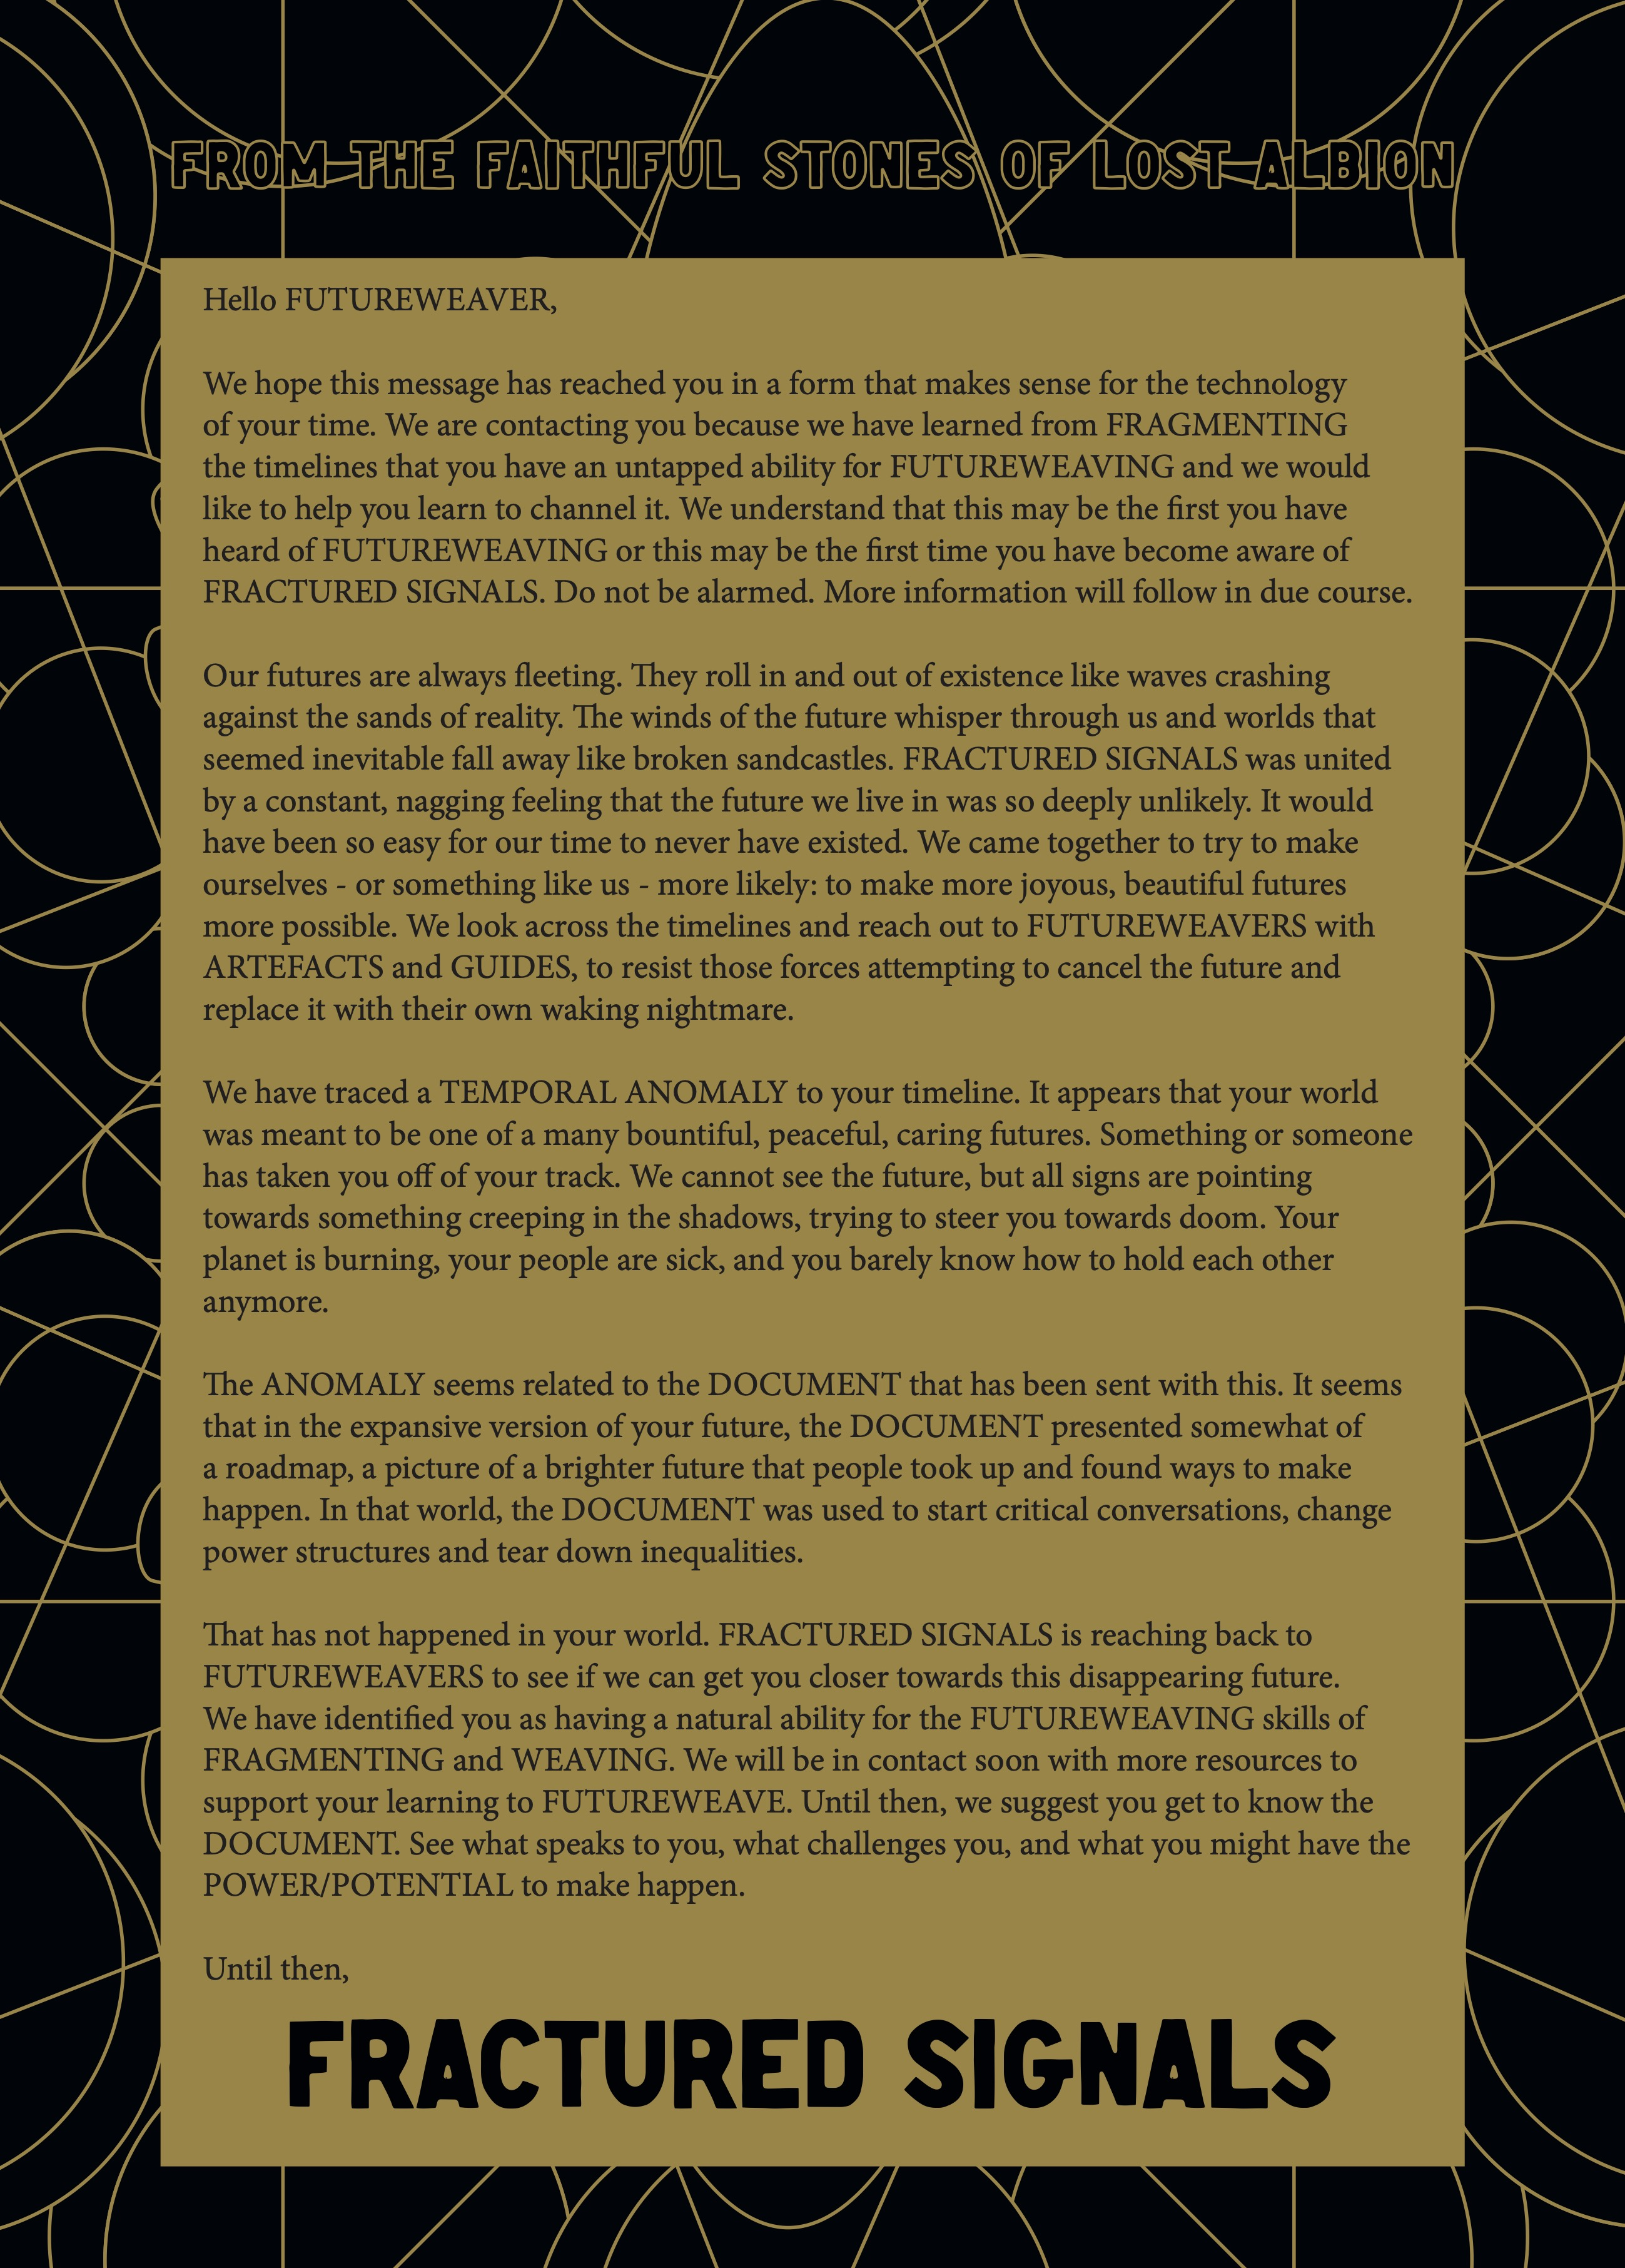
\includegraphics[width=1\linewidth]{Images/8/fs-letter.jpg}
    \caption{One version of the invitation letter that participants were sent}
    \label{fig:fs-invitation}
\end{figure}

\begin{figure}
    \centering
       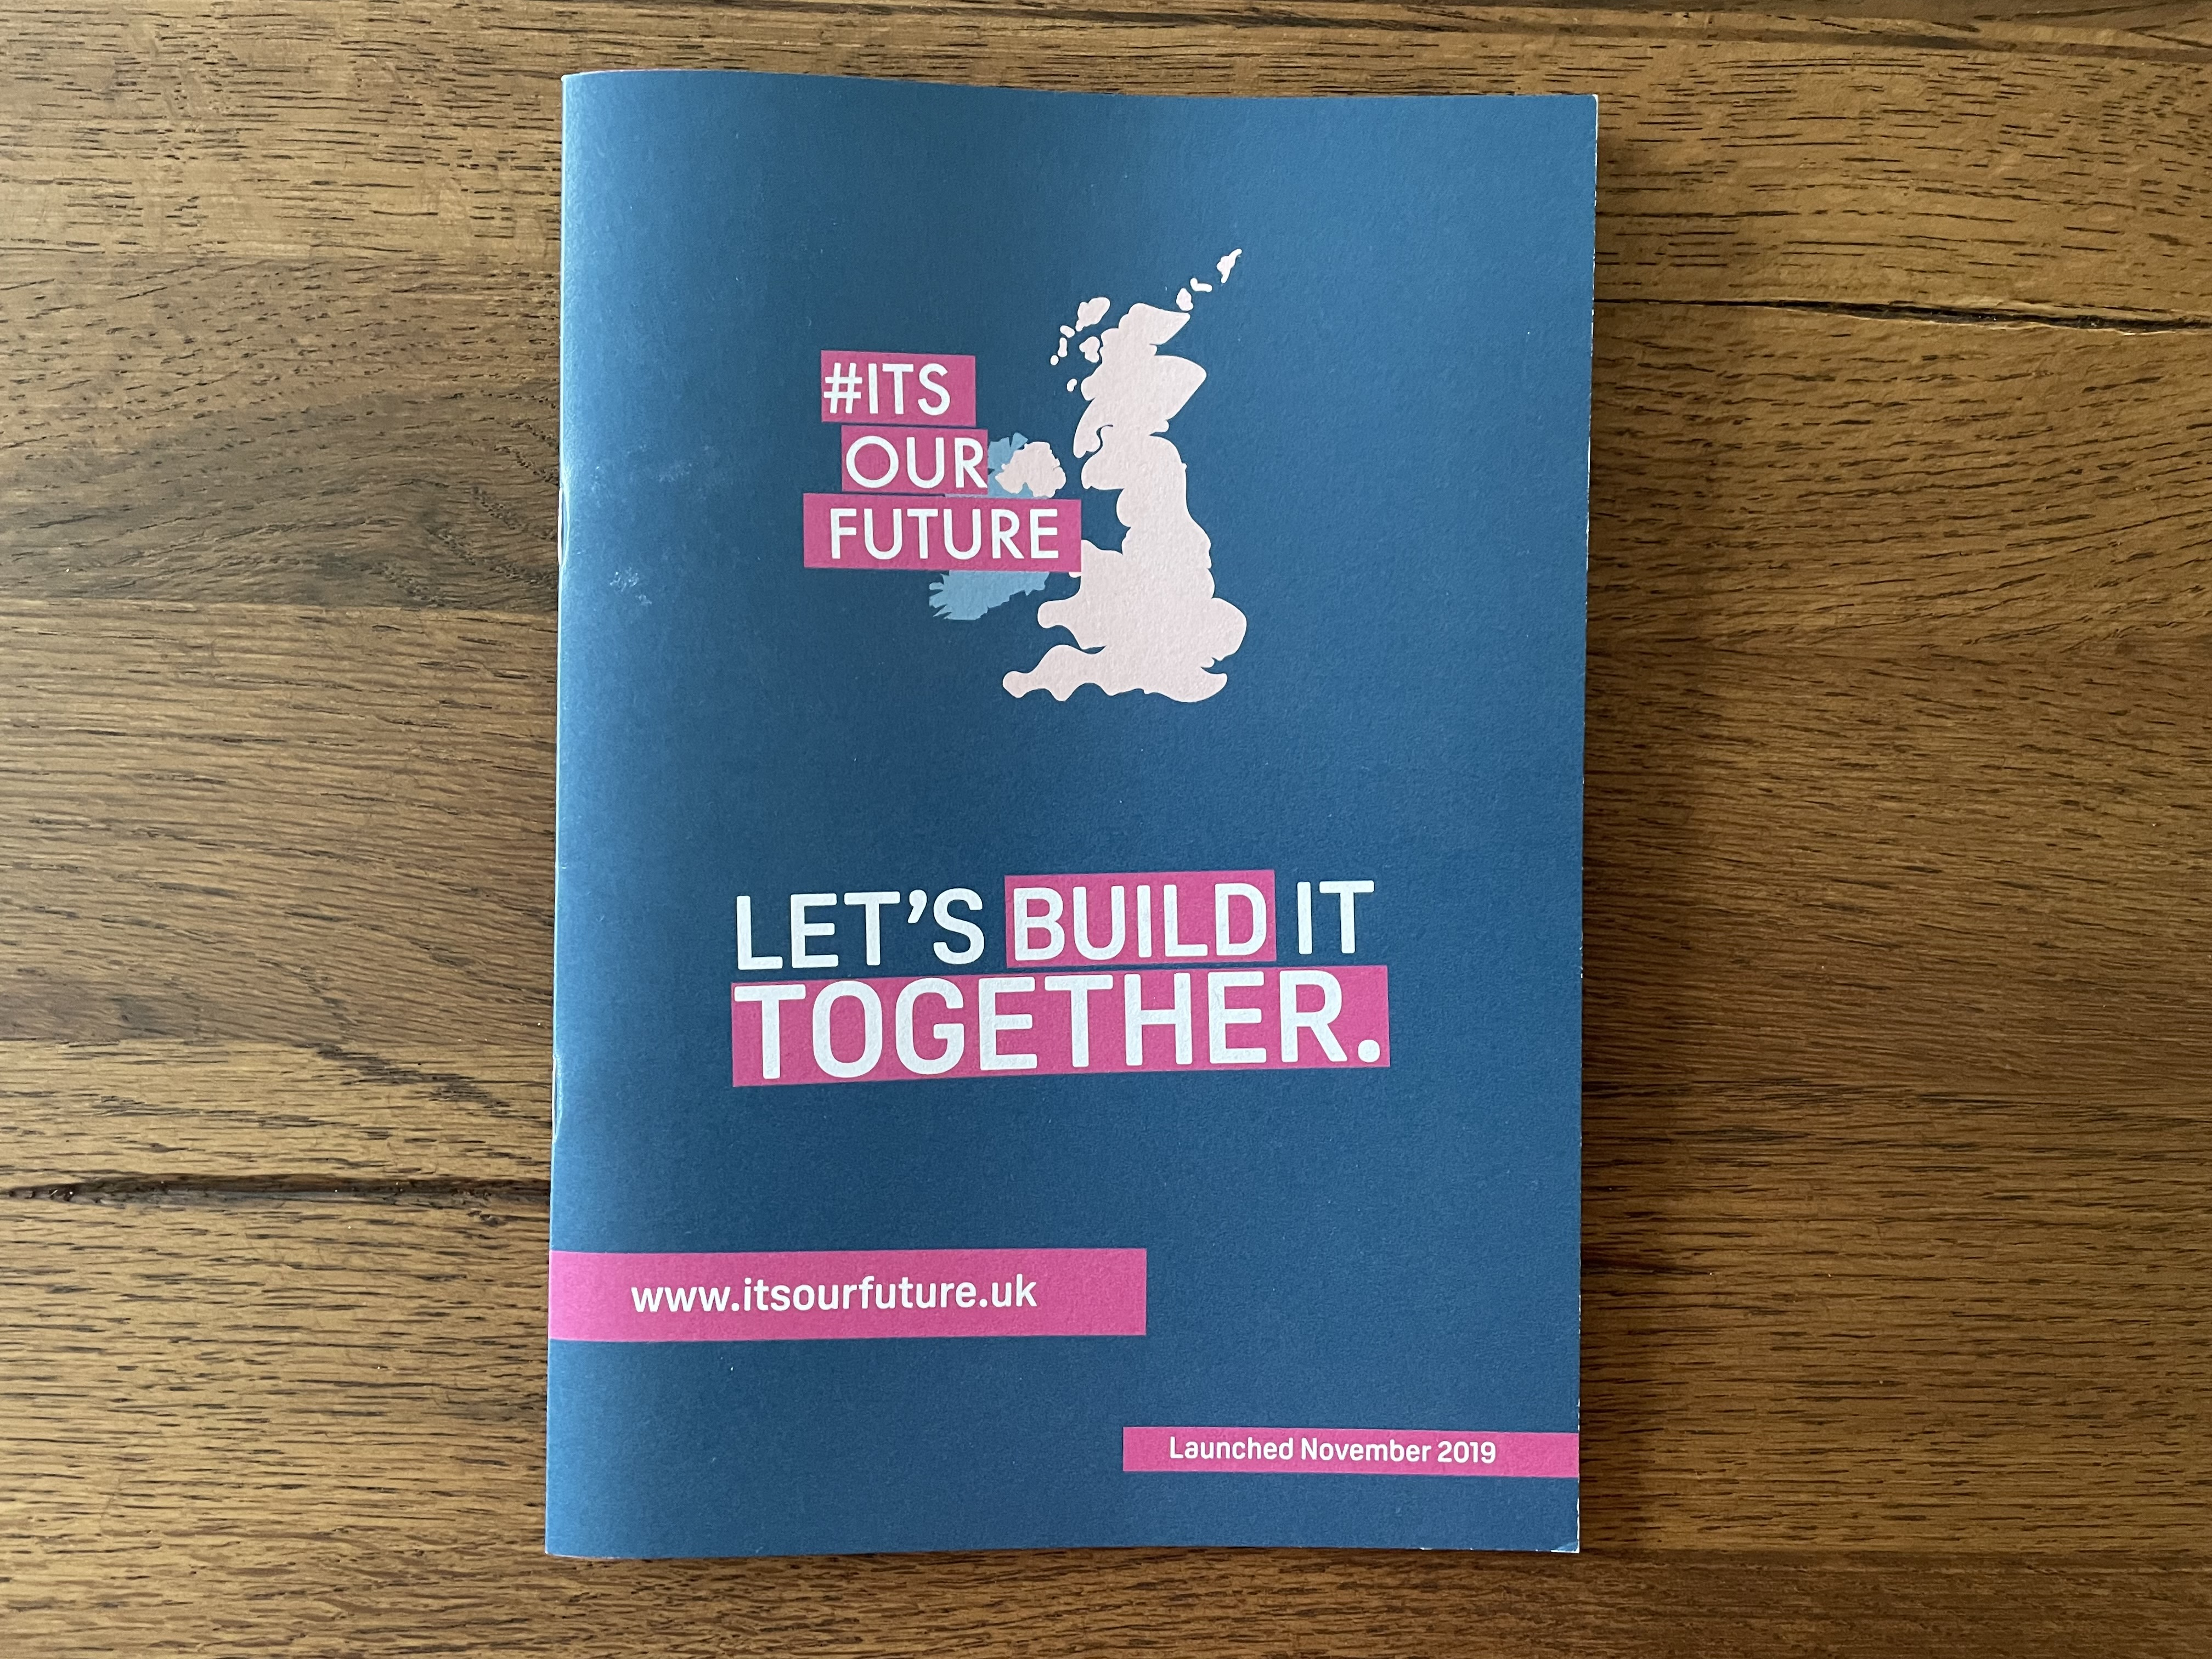
\includegraphics[width=1\linewidth]{Images/8/fs-doc.jpg}
    \caption{The printed \emph{It's Our Future} manifesto, sent to participants as 'the document'}
    \label{fig:fs-document}
\end{figure}

\subsection{The dreamthreads and divining board}
\label{subsedc:8-4-2-dreamthreads}
The core diegetic prototype used within the project was the 'dreamthreads' (a set of custom-designed tarot cards) and the divining board (a tool for using the dreamthreads without assistance). As referenced earlier, we knew that we wanted to use a form for the diegetic prototypes that communicated a visual language associated with reading and making futures. The tarot form felt additionally suitable because of the tarot's existing use in self-reflection processes, as people who use it tend to pull and consult tarot cards daily or when experiencing a problem in their lives. We designed these 22 cards around the 'major arcana' of the tarot, a series of 22 cards comprising evocative archetypes. The major arcana is also referred to as the fool's journey, as it tracks the progression of a mind through the stages of seeking self-knowledge, from the first card ('The Fool', the card of beginnings and naivety) to the last card ('The World', the card of fulfillment and integration).  We tried to draw on the feeling of ritual associated with the tarot as a design resource. We referred to the cards as dreamthreads within the project as they were meant to be abstract representations of moments of individual people's dreams. In the guide, fractured signals describe that the cards should:
\begin{quote}
feel like shards of something half-remembered. Something that might have been true, was true, or might be true at some point. We harnessed moments of our collective dreams across the timelines and have used these to represent some essential forms. 

These cards can help you in your early FUTUREWEAVING practice by taking the place of some aspect that you are holding in mind. It can be difficult to hold these in mind and visualise some part of the future at the same time. Let the DREAMTHREADS stand in. Use them however helps you to feel comfortable with them. The DIVINING BOARD contains some suggested uses, but these are not the only possibilities. We suggest working with the cards daily.    
\end{quote}
I held a design session with Daniel in which we explored traditional tarot iconography around each of the cards of the major arcana, and explored how these were expressed in different decks of tarot cards (shown in figure \ref{fig:tarot-design}). We then explored how the semantic field or imagery associated with each card could correlate to some aspect of the \emph{It’s Our Future} manifesto. To do this, we identified 22 substantive themes within the It’s Our Future research, drawing from the idea cards and manifesto primarily, and  mapped these against the 22 cards of the major arcana. We paired themes from the research with meanings of cards in the major arcana to give us a new deck of tarot cards which occupied the interpretative space of both things (detailed in table \ref{tab:tarot-meaning}). For example, 'The World' card in the tarot corresponds to 'The Explorer' card in the \textit{fractured signals} dreamthreads. ’The World’ card is typically associated with completion, integration, accomplishment and travel. It is the completion of the Fool’s Journey -  representing finishing what was started in ‘The Fool’ card. As ‘The Fool’ is a card of new beginnings, though, there is a sense that the cards are caught in a cycle of eternal recurrence, where 'The Fool' will ascend to the level of self-knowledge requisite in 'The World', only to begin again, starting anew. For us then, 'The Fool' became ‘The Fresh Start’, a card associated with moving away, being somewhere different, a chance to find yourself in a new place. ‘The Explorer’ on the other hand depicts the same character, subtly changed, embedded in a series of portraits at themselves. The card hints at the movement through time, the beginning of another cycle – but as an explorer, someone who goes to new places, demonstrates a level of commitment and confidence to experiencing the new. 'The Explorer' is 'The Fresh Start' with all of the knowledge of the Fool’s Journey. 

\begin{figure}
    \centering
    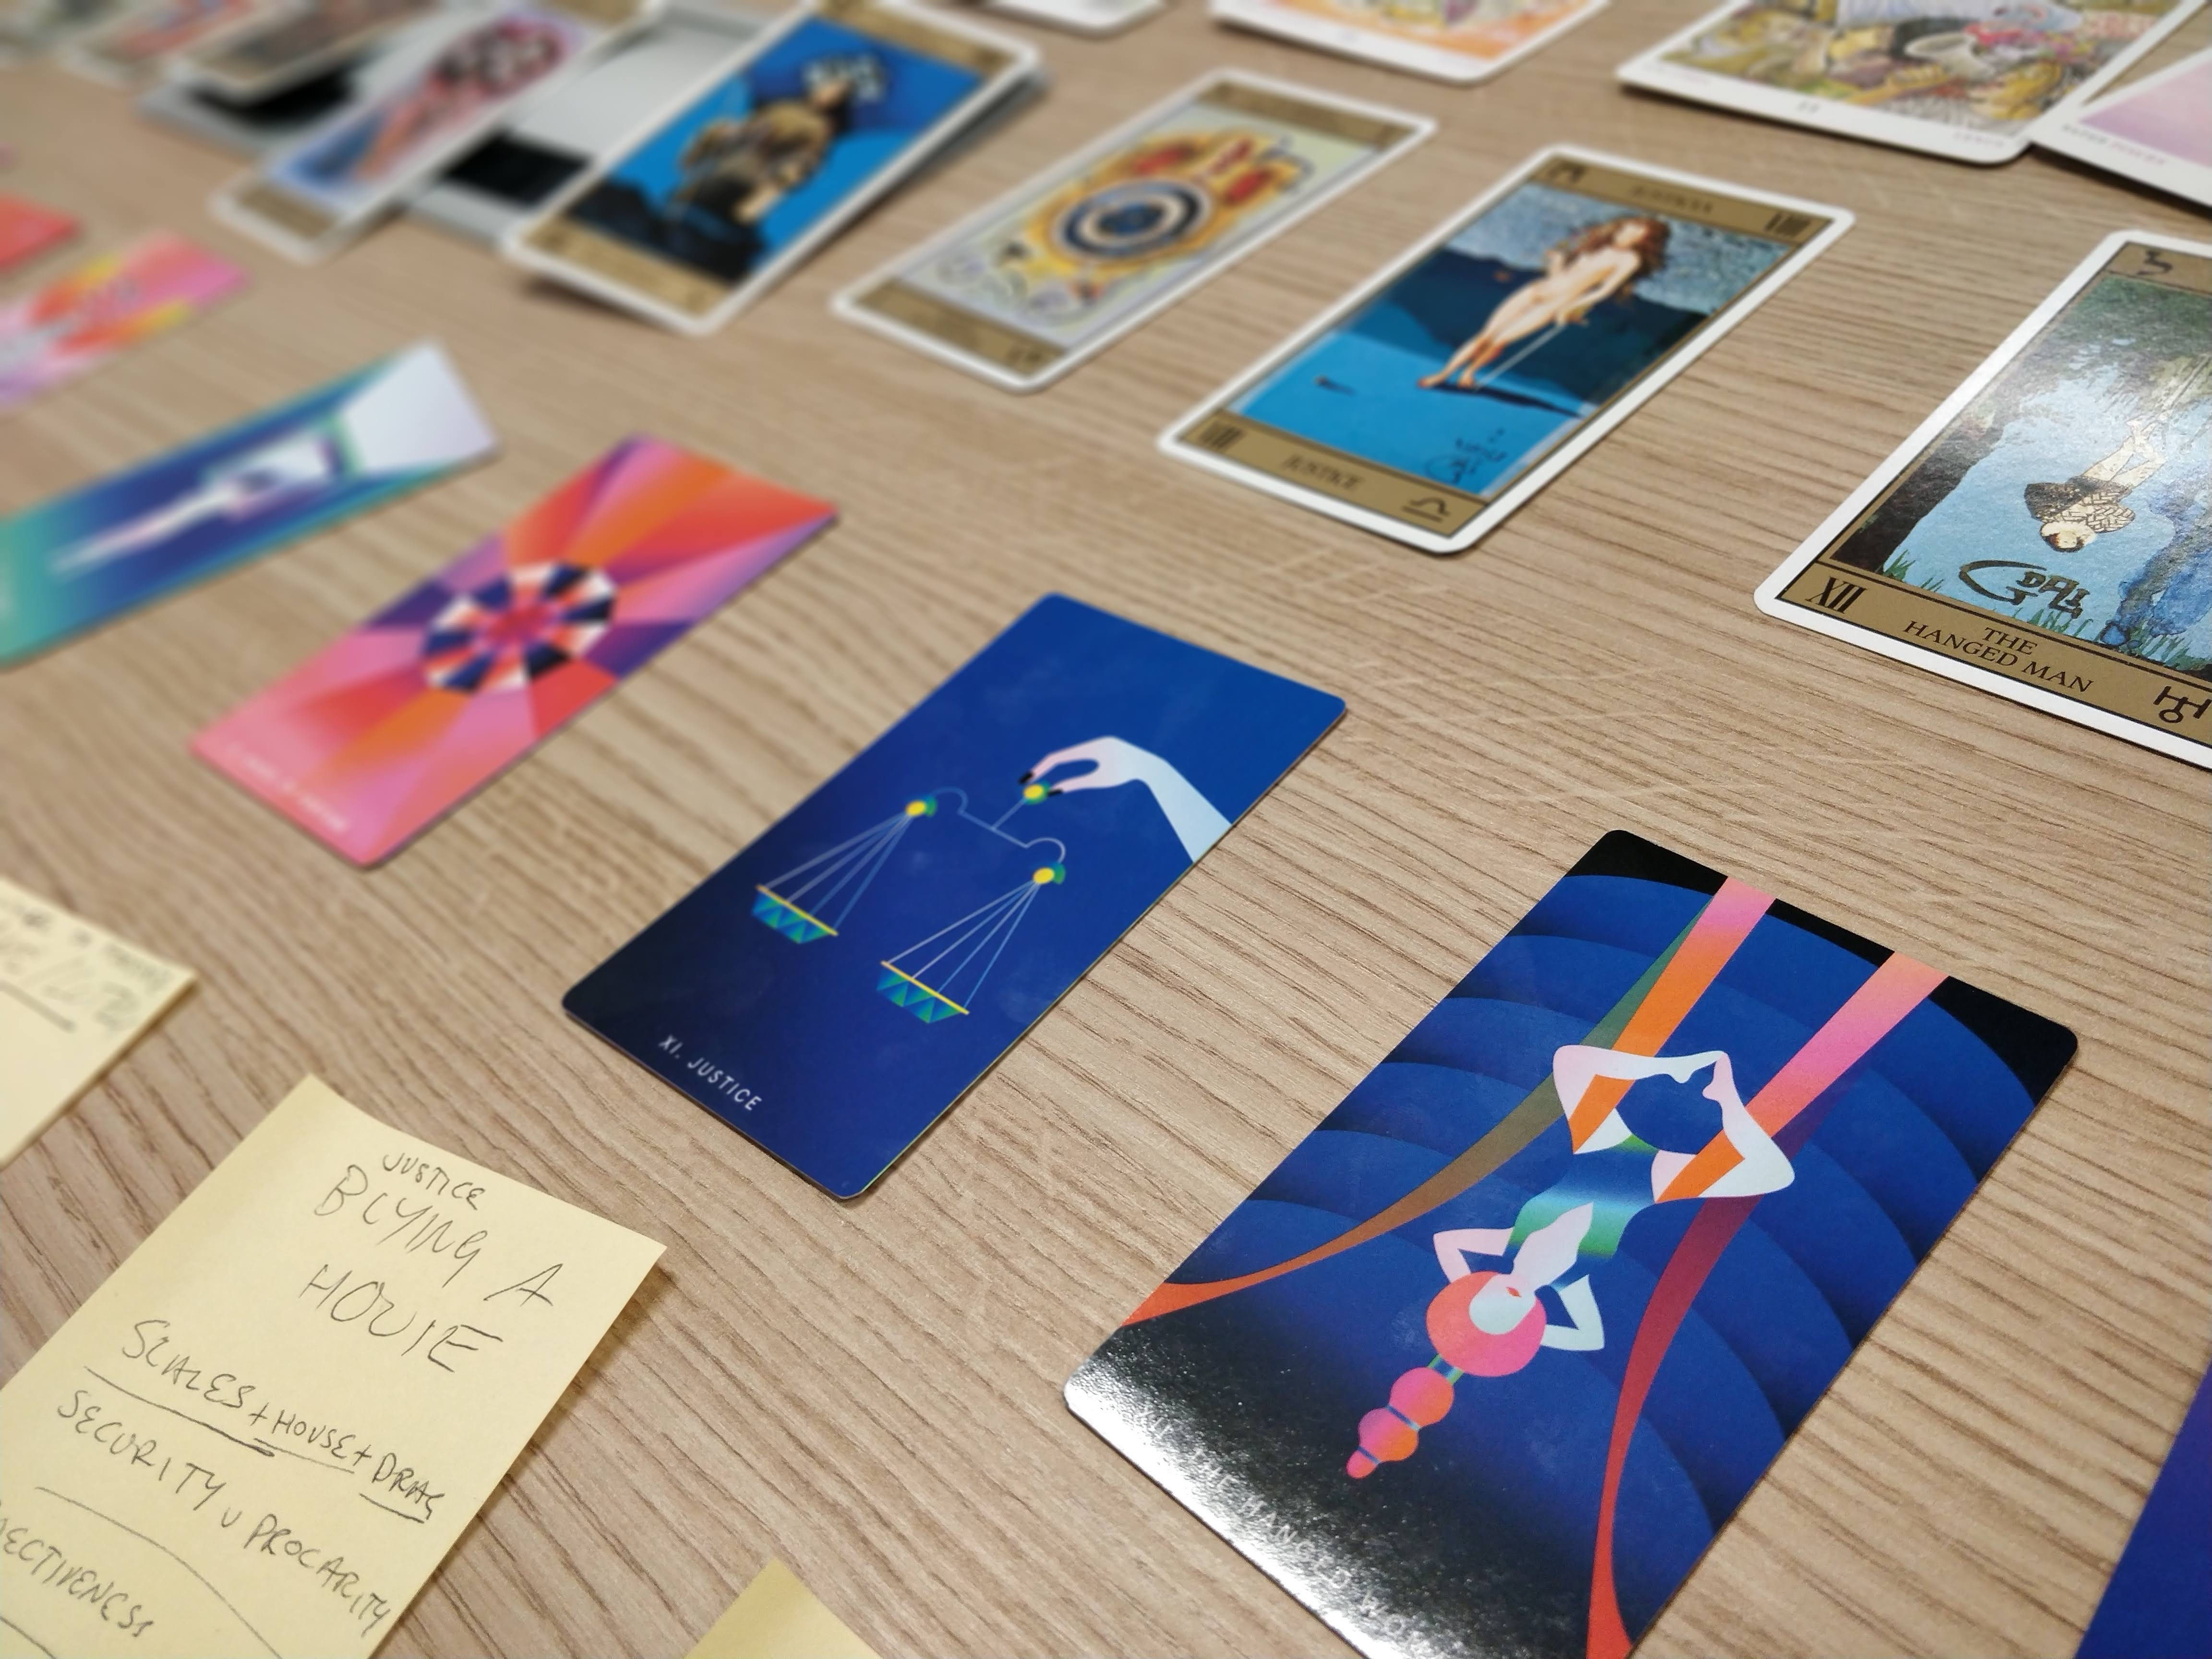
\includegraphics[width=1\linewidth]{Images/8/tarot-design-1.jpg}
    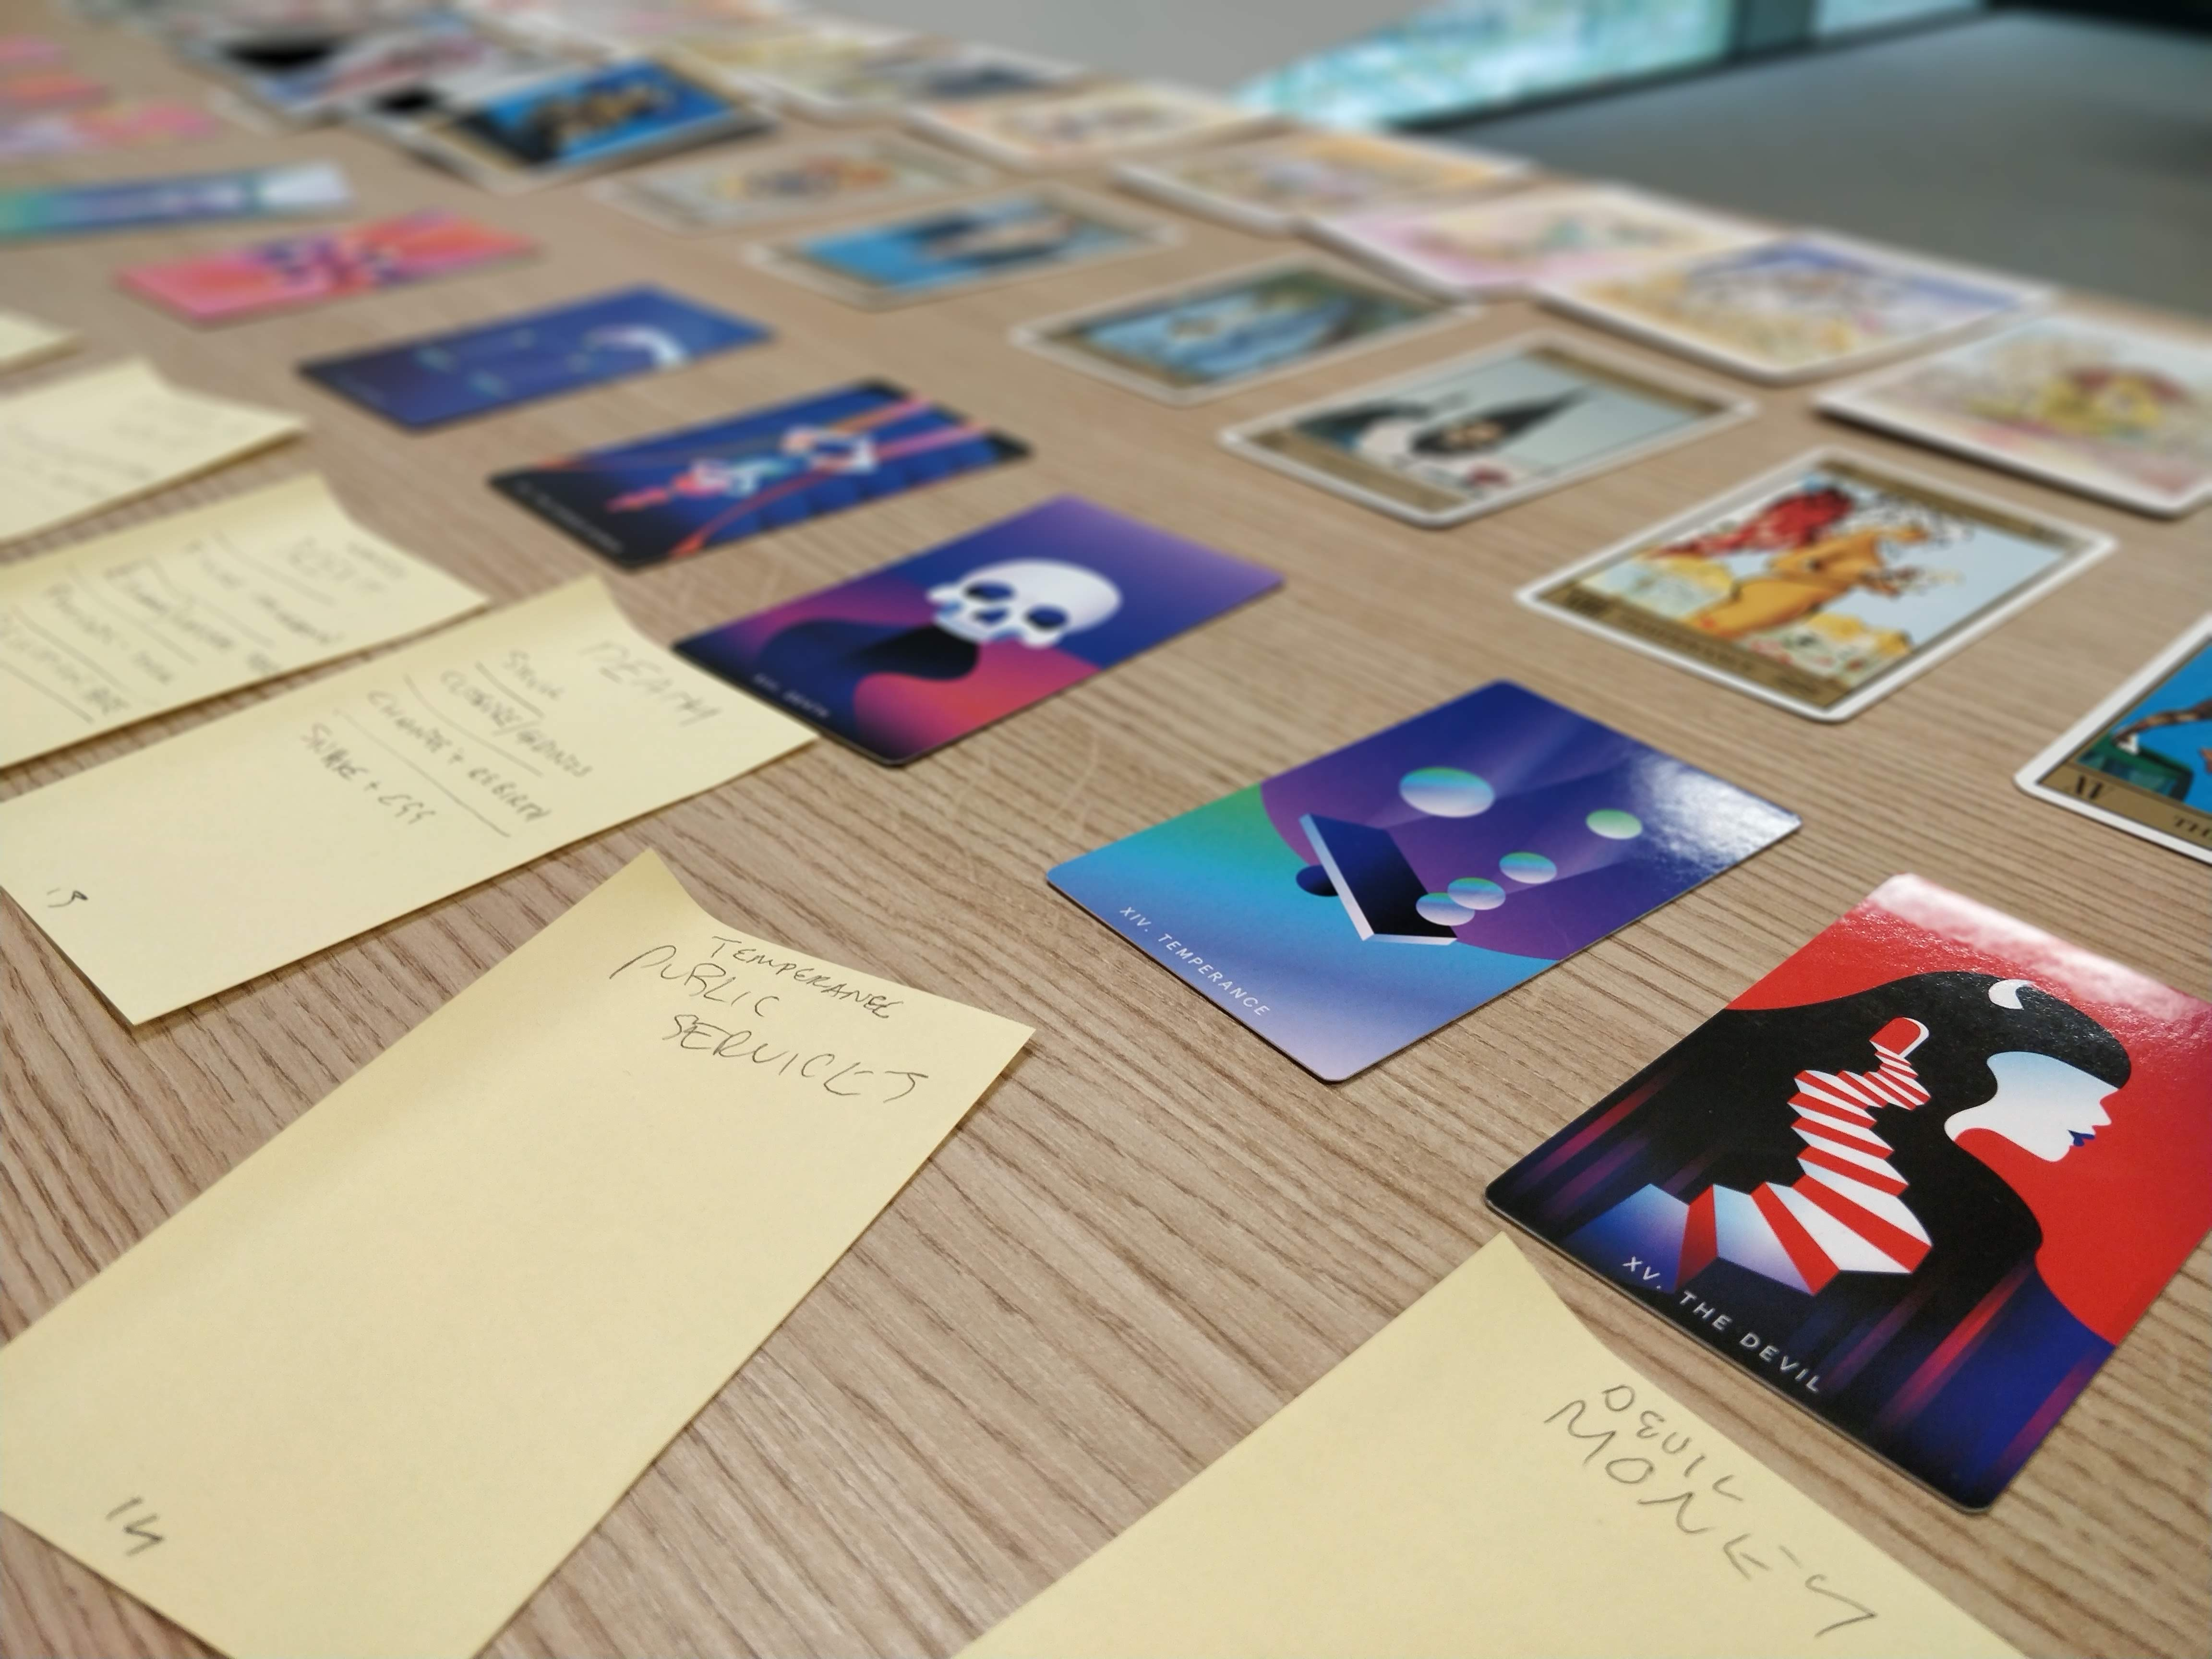
\includegraphics[width=1\linewidth]{Images/8/tarot-design-2.jpg}
    \caption{The tarot design session, featuring three different decks of tarot cards and our notes on iconography.}
    \label{fig:tarot-design}
\end{figure}

\begin{table}[]\hyphenpenalty=10000
\renewcommand{\arraystretch}{1.1}
\small
\resizebox{\columnwidth}{!}{%
\begin{tabular}{|>{\raggedright}p{1.5in}|>{\raggedright}p{2in}|>{\raggedright}p{1.5in}|>{\raggedright}p{2in}|}
\hline
\textbf{Card name in the tarot} &
  \textbf{Meaning} &
  \textbf{Card name in \textit{fractured signals}} &
  \textbf{Supporting data from \textit{It's Our Future}} \\  & \hline
The Fool         & beginnings, innocence, spontaneity                      & The Fresh Start      & Moving to somewhere new                               \\ & \hline
The Magician     & inspired action, resourcefulness, manifestation         & The New Voter        & Votes at 16                                           \\ & \hline
The High Priestess &
  intuition, the feminine, the subconscious &
  Fluidity &
  Greater gender equality and acceptance of gender non-conformity \\ & \hline
The Empress      & beauty, nature, femininity, abundance                   & Abundance            & Being in nature                                       \\ & \hline
The Emperor      & fatherhood, authority, the establishment                & The Cyborg           & Technology exerts too much control                    \\ & \hline
The Hierophant   & spirituality, wisdom, tradition                         & The Professor        & Going to uni or reforming education                   \\ & \hline
The Lovers       & love, harmony, choices                                  & The Family           & Having a good relationship with family                \\ & \hline
The Chariot      & control, willpower, action, determination               & The Motor            & Learning to drive                                     \\ & \hline
Strength         & strength, courage, influence                            & The Entrepreneur     & Having a job or starting a business                   \\ & \hline
The Hermit       & soul-searching, introspection, solitude, inner guidance & The Lost Identity    & Knowing yourself                                      \\ & \hline
Wheel of Fortune & good luck, destiny, turning points                      & The Sweepstakes      & Winning the lottery or becoming famous                \\ & \hline
Justice          & justice, fairness, truth, law                           & The New House        & Having secure housing or buying a house               \\ & \hline
The Hanged Man   & pause, surrender, letting go, new perspectives          & The Indefinite Pause & Stopping Brexit                                       \\ & \hline
Death            & endings, change, transformation                         & Decay                & A loved one dying                                     \\ & \hline
Temperance       & balance, moderation, patience, purpose                  & The Cup              & Well-funded public services                           \\ & \hline
The Devil        & shadow self, attachment, addiction                      & The Banker           & The rich are too powerful                             \\ & \hline
The Tower        & sudden change, upheaval, chaos, revelation              & The End              & A sudden end to the world                             \\ & \hline
The Star         & hope, faith, purpose, renewal                           & The Lighthouse       & Helping other people (e.g. refugees, homeless people) \\ & \hline
The Moon         & illusion, fear, anxiety, subconscious, intuition        & The Mind             & Better mental health support                          \\ & \hline
The Sun          & positivity, fun, warmth, success                        & The Future           & Feeling confident about the future                    \\ & \hline
Judgement        & judgment, rebirth, inner calling, absolution            & Absolution           & Addressing the climate crisis                         \\ & \hline
The World        & completion, integration, accomplishment, travel         & The Explorer         & Exploring the world  \\ & \hline                                  
\end{tabular}%
}
%
\caption{A table displaying the cards of the major arcana, their meanings, the card's name in \textit{fractured signals}, and the data from \textit{It's Our Future} this was drawn from.}
\label{tab:tarot-meaning}
\end{table}

By adapting the cards in this way, we were able to craft a visual language that drew connections from \emph{It's Our Future} abstractly into \emph{fractured signals} and gave insight to deeper nuances about the data collected from \emph{It's Our Future}. ‘The Cyborg’, for example, is ‘The Emperor’ in the tarot, which is a card about paternalism, authority and the establishment - a card that might represent control, restriction, or the way that things have always been done. This idea of control was mirrored in the ways that young people who attended \textit{It’s Our Future} felt about technology – that it was something removing their control and making them feel as if they had no agency over their usage of, or participation in the wider changes being made by technology. In making ‘The Emperor’ into ‘The Cyborg’, we begin to suggest that perhaps technology has become our new rulers, or that the establishment has simply taken on the clothes and framing of the technological in order to find new ways to enact their control. This expanded visual semantic field enhanced the range of meanings of each card and enabled them to act as ambiguous resources for reflection. Each card contained iconography referring to the original representation within the tarot and the \textit{It's Our Future} data, giving more threads for people to draw upon in their reflections. The\textit{ fractured signals} cards ensure that the meaning of the tarot is comprehensible within the contemporary context of the experiences and desires of young people perceived to be vulnerable. Each of the cards can be seen in figure \ref{fig:dreamthreads}

\begin{figure}
    \centering
    \includegraphics[width=0.9\linewidth]{Images/8/allcards.png}
    \caption{Each of the \textit{fractured signals} dreamthreads.}
    \label{fig:dreamthreads}
\end{figure}

The dreamthreads could either be used under the instruction of fractured signals (during the phone calls), or on their own, as a reflection tool. As each card represents a fragment of meaning from \textit{It’s Our Future} participants could think about what the card represented to them and what potential meanings it might have, guided by the questions in the guide. They could also be used in a problem-led sense - if participants were having trouble with an issue in their work, they would be able to draw a card at random and reflect on the advice it might have suggested to them. In both the self-directed and fractured signals-led uses, the dreamthreads could be used in combination with the divining board, which suggests some potential contexts for each of the cards to be considered within (pictured in figure \ref{fig:divining-board}). These were adapted from common tarot card spreads, which give a logic and consistency to how randomly chosen tarot cards can be made to make sense. Examples include ‘past, present, future’, and ‘context, problem, lesson’. Each card pulled in order would give some specifically tailored reflection on the participant's current situation. I developed the divining board as a support tool for participants who might not easily understand that each card could play a specific role in a reflection process, and to further add to the fiction that fractured signals had contacted the participant in order to provide them support tools in their futureweaving journey.
\begin{figure}
    \centering
    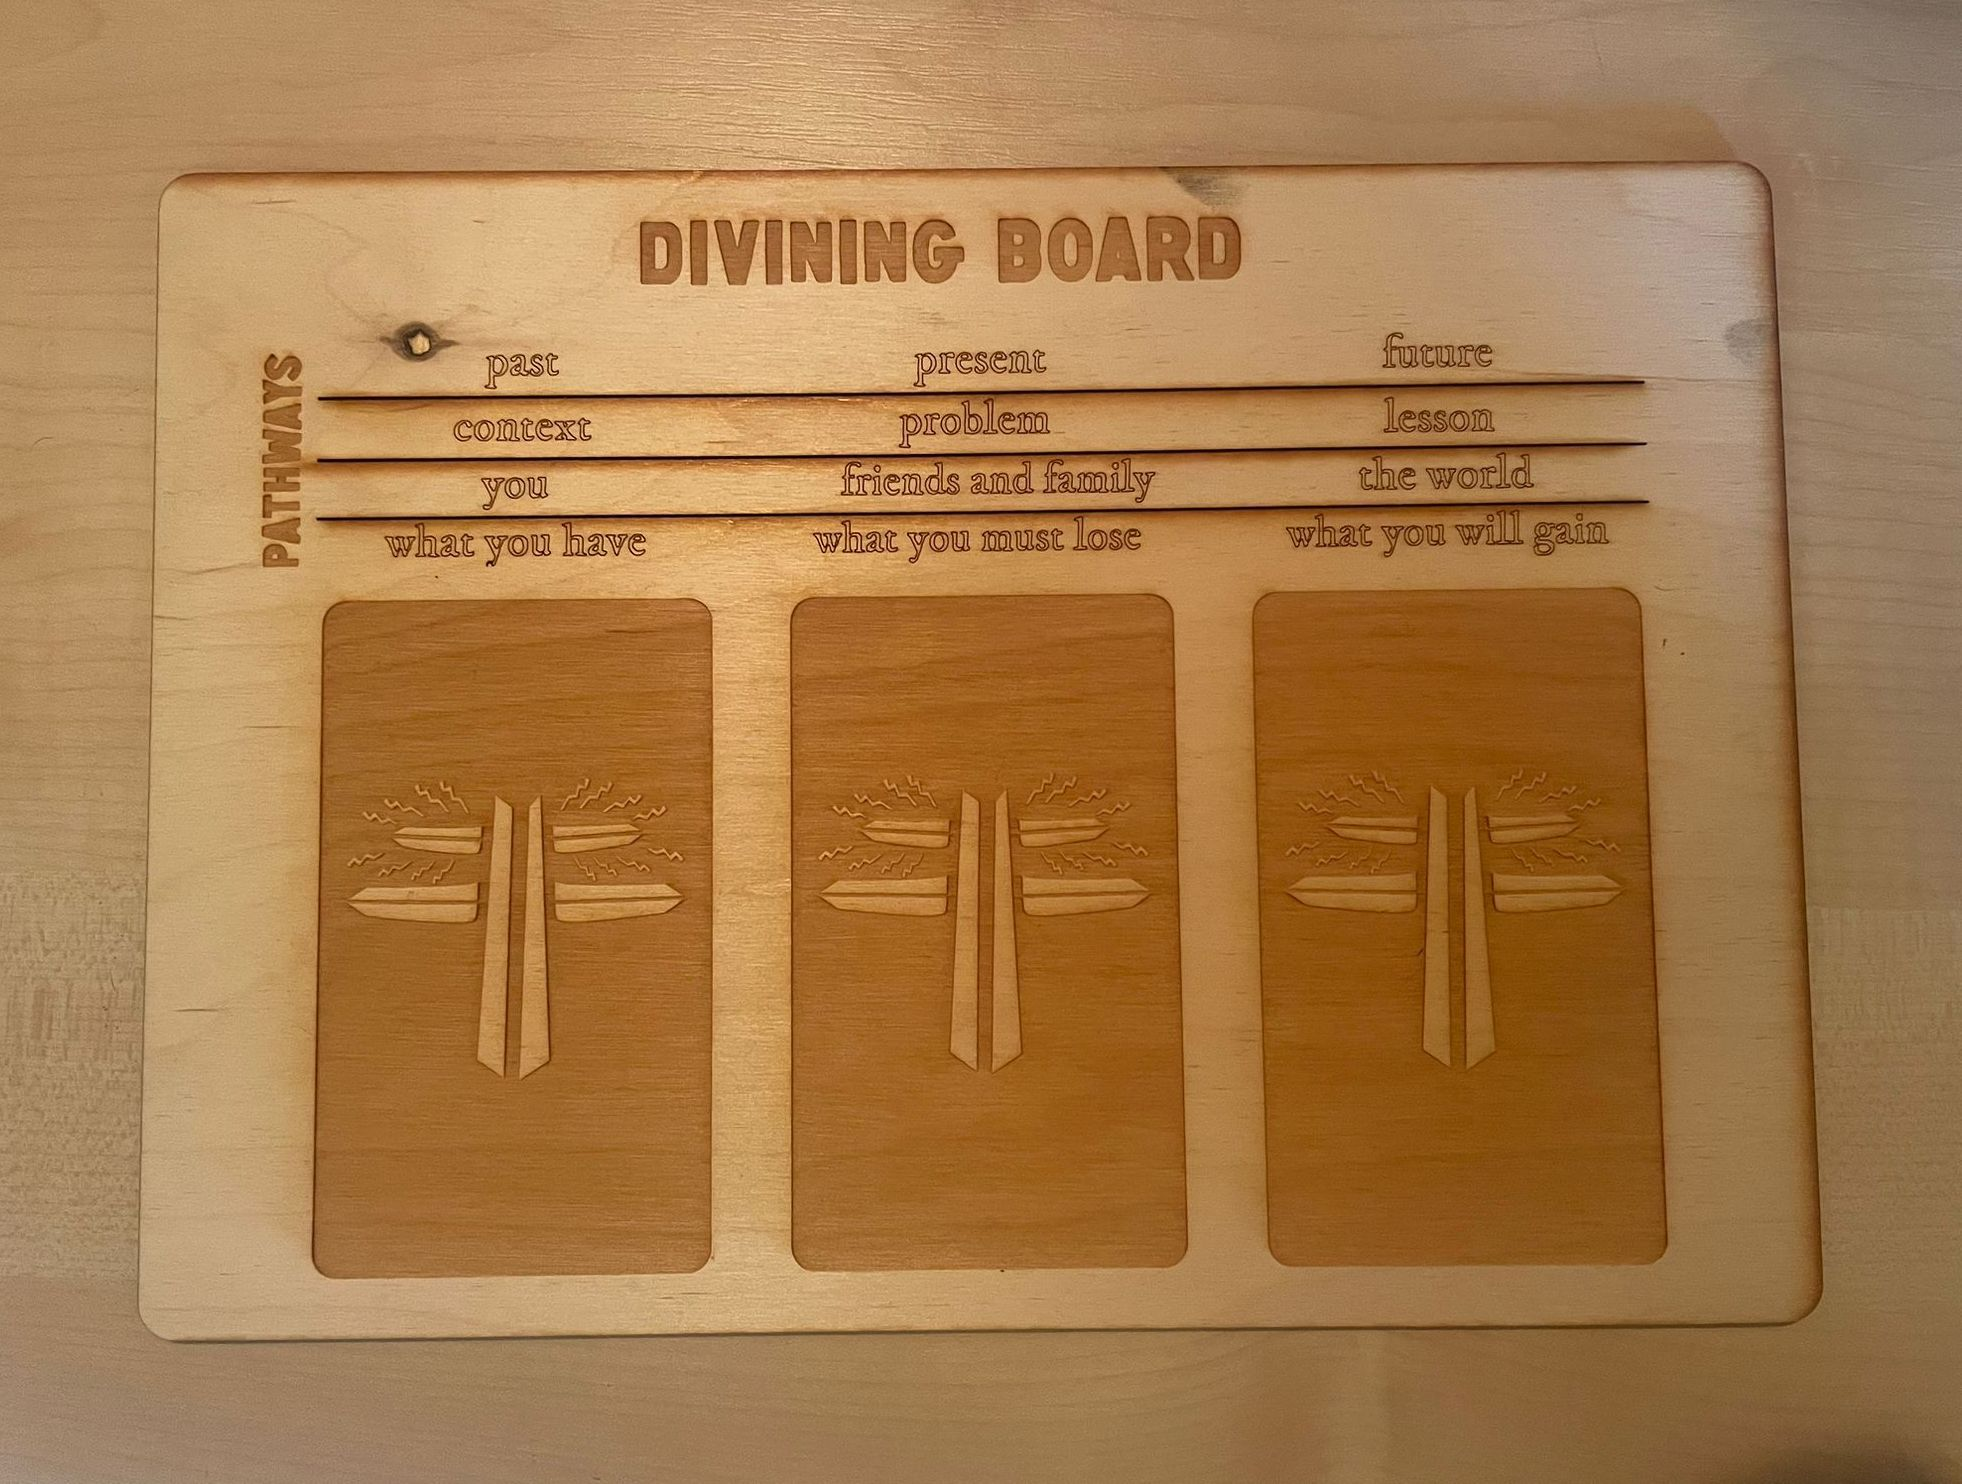
\includegraphics{Images/8/divining-board.jpg}
    \caption{The divining board used in \textit{fractured signals}}
    \label{fig:divining-board}
\end{figure}

\subsection{A Guide for New Futureweavers}

A week after the invitation arrived with participants, the rest of the artefacts were sent to them. \textit{A Guide for New Futureweavers} explained each of the artefacts, brought them further into the fiction, and helped participants to gain a sense of what each of the diegetic prototypes were and how to use them. The \textit{Guide} began with a description of the multiple futures that fractured signals exists across, before detailing who fractured signals are, and what futureweaving is. Then, the \textit{Guide} described each of the artefacts in depth – giving potential meanings for each of the dreamthreads, showing how to use the divining board, and how to operate the signalfinder. 

The opening pages describe the contingency of the multiple futures that fractured signals exist across (shown in figure \ref{fig:guide}).  My intent here was to begin troubling the notion of linear progression of time, and to start creating a sense of possibility, building on the idea that the singular, capitalist realist notion of the future is just one potential future and that there is an alternative. In doing so, I worked on the strategies of ‘richly imagining possible futures’, ‘make our current world seem strange or distant’, and ‘make future worlds seem more possible’.  After this, the \textit{Guide }introduced fractured signals as a far-future multi-timeline organization that may or may not exist (also shown in figure \ref{fig:guide}). By deliberately invoking its own fictionality in this way, participants would be called to consider the gap between reality, fiction and possibility. This semi-fictionality brought them deeper into the world of the speculative enactment. The \textit{Guide} also existed as a resource for participants to draw on after the engagement process was over, containing potential meanings and questions for each of the dreamthreads cards.

\begin{figure}
    \centering
    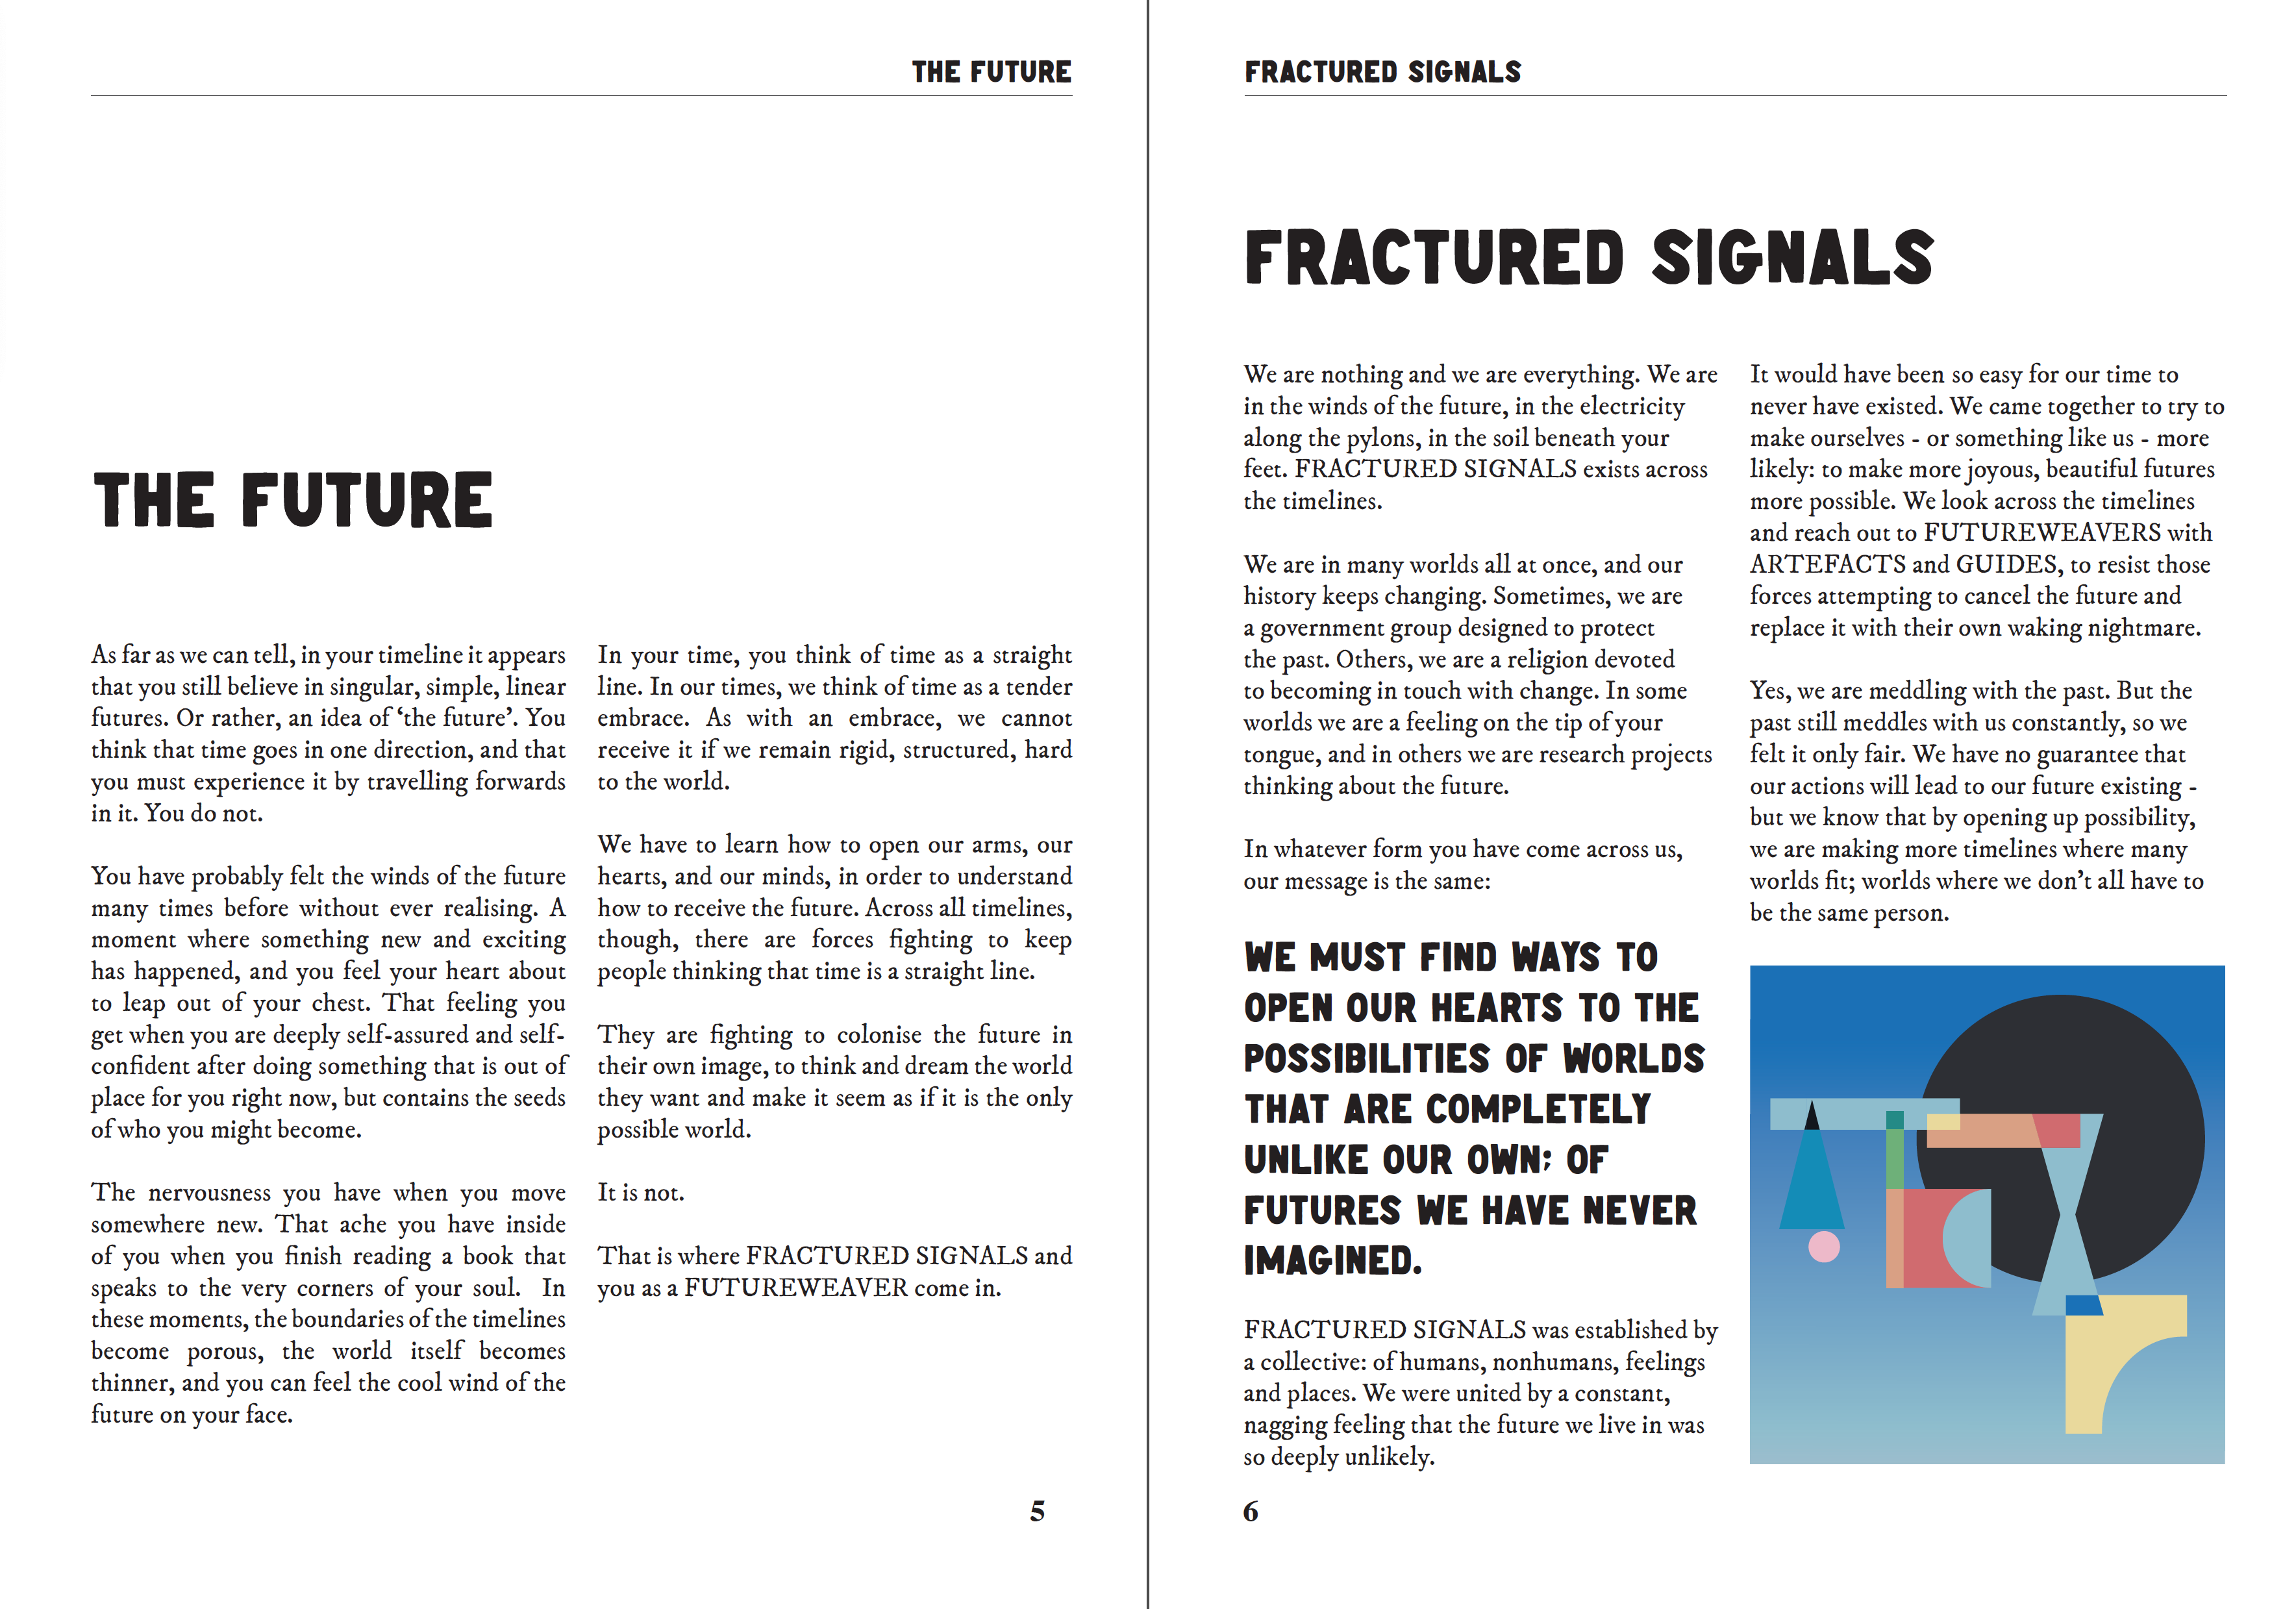
\includegraphics[width=0.9\linewidth]{Images/8/guide-1.png}
    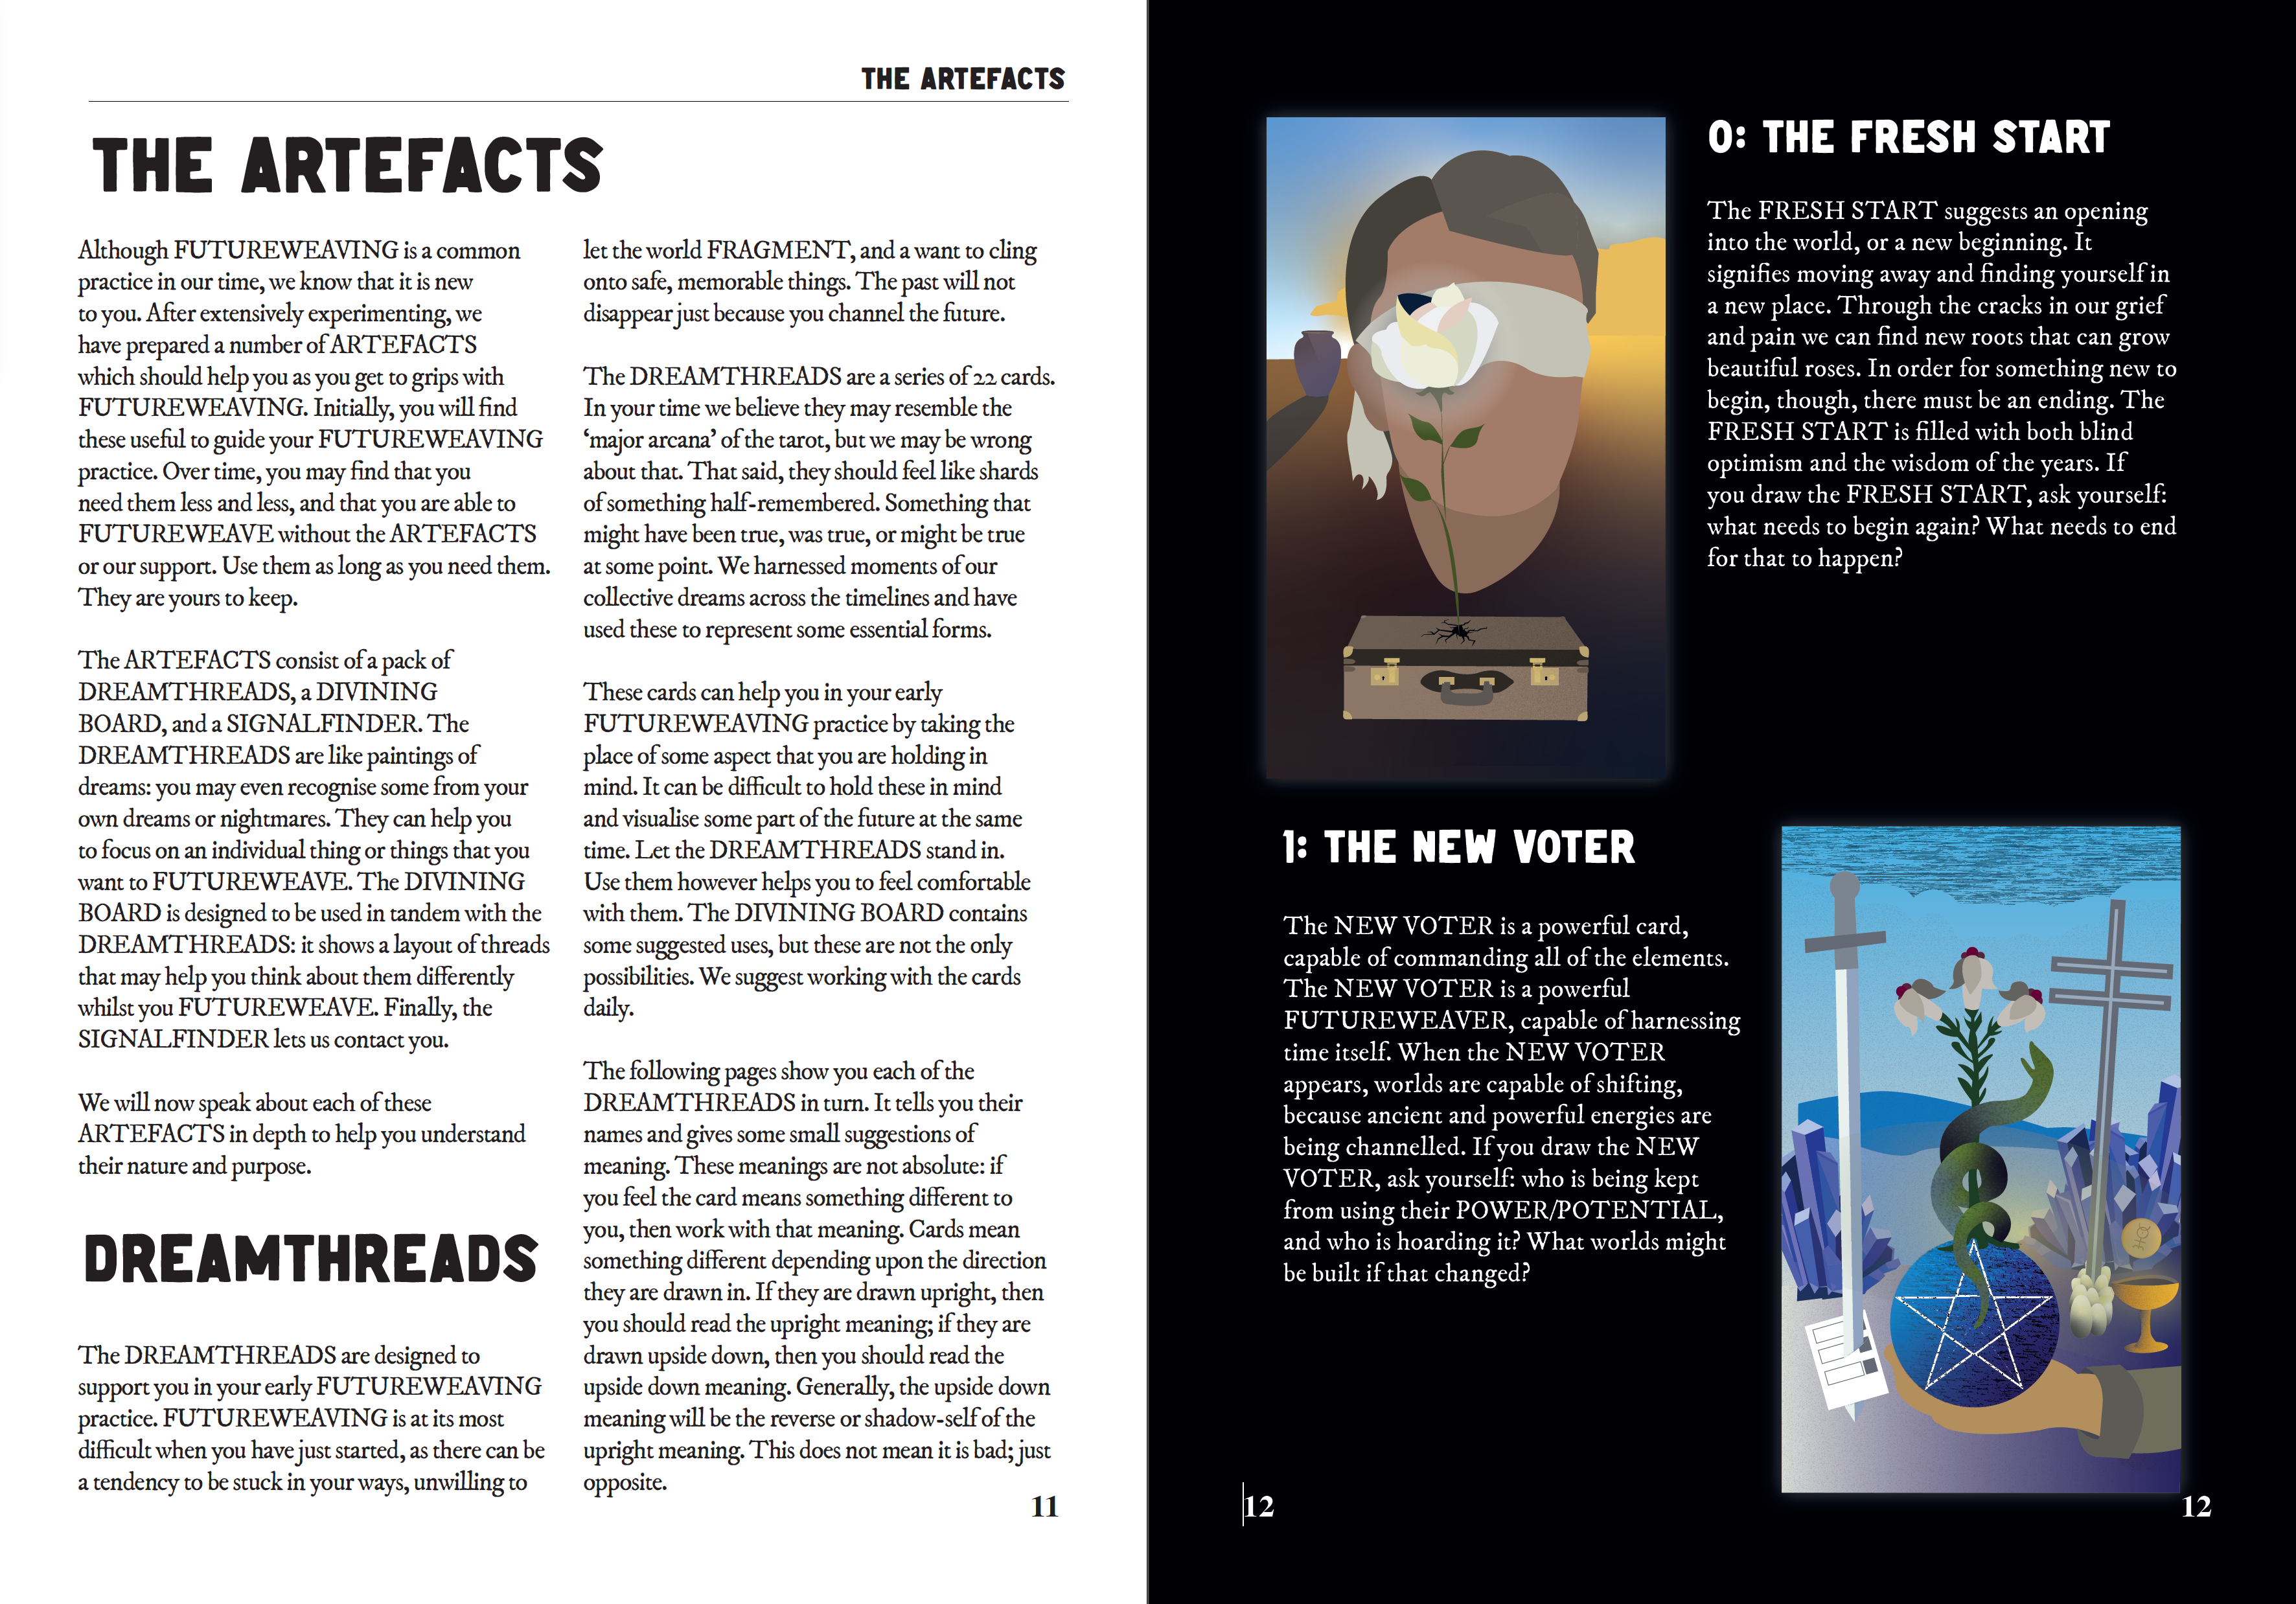
\includegraphics[width=0.9\linewidth]{Images/8/guide-2.png}
    \caption{A selection of pages from \textit{A Guide for New Futureweavers} which talks participants through a different idea of the future, introduces fractured signals, and presents the diegetic prototypes as artefacts.}
    \label{fig:guide}
\end{figure}


\subsection{The signalfinder}

The last diegetic prototype was the signalfinder, a small wooden box that was designed both to house the cards and act as a passive speaker for participants’ phones when they called the fractured signals phone number (pictured in figure \ref{fig:signalfinder}). The box went through a number of designs before landing on this final design, mostly requiring adjustments because of issues with the living hinge around the side (a prior iteration is shown in figure \ref{fig:prior-box}). In its final design, the dreamthreads sit inside of the box, and most sizes of modern mobile phone rest easily on the phone stand on the top of the box. Assuming that the phone’s speakers are on the base (as most are), the spaces in the living hinge at the front create a small degree of amplification for sound coming out of the phone’s speakers. Whilst this was one of our central aims for the design of the signalfinder, the amplification was very small and not likely to make a huge difference for participants. 

The key design aspect of the signalfinder was its role as a diegetic prototype that brought participants further into the speculative enactment. In the narratuve of the project, the signalfinder is essential for contacting fractured signals through a regular phone call, as the organisation needs the participants to use the signalfinder in order to locate them through different possible timelines. In the narrative, the signalfinder amplifies "resonant frequencies" through different timestreams to make it easier for fractured signals to locate participants. By making the signalfinder into a passive speaker, I played with this idea of aural resonance, audio compression through phone calls (signal loss), and connected it to the idea of temporal resonance and the fracturing of signals from the past. Mostly, I hoped that the ritual of taking the cards out of the signalfinder, setting up the stand, placing the phone on top of the stand and calling fractured signals would help slowly create a narrative space for participants to feel as if they were entering the world of fractured signals. 

\begin{figure}
    \centering
    \includegraphics{Images/8/sigfnalfinder.jpg}
    \caption{The final design for the signalfinder box}
    \label{fig:signalfinder}
\end{figure}

\begin{figure}
    \centering
    \includegraphics{Images/8/prior-signalfinder.jpg}
    \caption{A prior design for the signalfinder box, that did not result in any passive amplification}
    \label{fig:prior-box}
\end{figure}


\subsection{Phone calls (through Twilio)}

Participants were given the instruction to call a certain phone number each day during the engagement process. On the other end of the phone, a series of robotic voices would speak the script that I had written, which guided them through interactions with the other artefacts (centrally, the dreamthreads and divining board). As previously explained, each day of the engagement process focused on a different intended outcome based around the methods featured in table \ref{tab:fs-methods}. Fragmentation day 2 and 3 do not feature in this table because they were aspects of the engagement that were not based in prior methods explored in either \textit{It's Our Future} or \textit{Design Strategies against Justification Practices}, and were more specifically focused on what was needed for the specific frame of the engagement. Day 2 focused on supporting workers to develop a deeper understanding of the young people they work with, whilst day 3 asked them to analyse and pay attention to the cards specifically. Day 3 was a research-specific task, trying to understand the different kinds of meanings participants project onto the cards.  

I wrote some code to handle the interactions through Twilio (available in appendix \ref{appendix:code}), a programmable communication tool. I wrote the script (available in appendix \ref{appendix:fs-script}) so that each day, the segment of script that the code was reading from would change. The voices were produced by Amazon Polly, a text-to-speech service that is integrated into Twilio, and every segment of the script was read by a randomised voice, so that no two participants would have the same set of voices. By basing these interactions on phone calls, I continued my strategy of having a low barrier to participation in the process as I was aware that all participants had access to a mobile phone through their work. The phone calls acted as another diegetic prototype, inviting people directly into the world of fractured signals by `speaking' to them on the phone, a means of asynchronous distance workshop delivery, and a convenient way to record data, as Twilio allows for the recording of voice messages. Within the project, participants were made aware that their interactions via phone calls would be recorded.

\section{Understanding the efficacy of the \textit{fractured signals} methods}
14 workers signed up to the \textit{fractured signals} project and nine people participated. Of these nine, two only participated for a single day. The remaining seven all called \textit{fractured signals} for most of the project, though one only called three times. In response to participants explaining that they had missed days due to busy work days, I also made it possible for participants to call on a weekend and participate in a day they might have missed. Most participants made use of this at least once. The participants in the project and their associated roles are listed in table \ref{tab:fs-participants}. Of these participants, Mandy, Karen, Frank were part of the Building Bridges project, whilst Penny also worked in The Charity. The other participants worked in other national charities or were student social workers.

\begin{table}[]
\centering
\begin{tabular}{|l|l|} \hline 
\textbf{Name (pseudonym)} & \textbf{Role}                    \\ \hline 
Mandy                     & Research Lead                    \\ \hline 
Karen                     & National Projects Co-ordinator   \\ \hline 
Frank                     & Mental Health Practitioner       \\ \hline 
Steve                     & Policy and Participation Manager \\ \hline 
Penny                     & Mentor                           \\ \hline 
Ellen                     & Student Social Worker            \\ \hline 
Rory                      & Student Social Worker           
 \\ \hline\end{tabular}

\caption{A list of significant participants in the \emph{fractured signals} project.}
\label{tab:fs-participants}
\end{table}
As explored earlier in this chapter and in the previous chapter, to develop effective methods of mitigating, resisting, or creative an alternative to austerity-intensified capitalist realism that is based in a worker-centric intervention, these methods must:
\begin{itemize}
\item reduce workloads or provide workers with the tools to navigate their workplaces more comfortably,
\item support workers to either do work they are skilled at, or to gain skills at an appropriate pace, or
\item build more trusting relationships between workers and managers, or reduce managers' use of control techniques.
\end{itemize}
Alongside this, to disrupt justification, classification and discursive accumulation practices that render work with young people perceived to be vulnerable tokenistic, these methods must disrupt:
\begin{itemize}
    \item  the prioritisation of evaluation (whether by skilled or unskilled evaluators),
    \item breaking projects up into granular outcomes and outputs, which are then used to justify the organisation's practice,
    \item  the stratification of support according to the (funding-linked) identities of young people, or
    \item  the production of 'best practice' and innovation through discursive accumulation.
\end{itemize}
Finally, disrupting austerity-intensified capitalist realism would involve countering the notion that  "capitalism is the only viable political and economic system" by making it possible to imagine a coherent alternative to it \citep{fisher_capitalist_2009}. In analysing the experiences that participants had throughout \textit{fractured signals}, I was looking for evidence that it supported change in one or several of these ways. I found that the methods were particularly effective at surfacing workplace issues and building work voice and power, envisioning futures that center alternative values, and centering the experiences of young people perceived to be vulnerable.

\subsection{Developing critical consciousness in the workplace}
Generally, the engagement process seemed to support the creation of critical consciousness in and about the workplace. Workers who participated in the project became more aware of the problems in their organisations, their own practices, and became bolder about wanting to do something about these. This was facilitated by several of the strategies employed within \textit{fractured signals}, including:
\begin{itemize}
    \item Supporting the development of critical consciousness,
    \item Identifying existing power dynamics and systemic issues,
    \item Making our current world seem strange or distant,
    \item Helping people to understand their assets, skills and resources,
    \item Facilitating skills exchange,
    \item Supporting healing through the process, and
    \item Creating effective onward action.
\end{itemize}

Throughout the project, Frank became more comfortable with acknowledging the dynamics of justification, classification and discursive accumulation, and his own complicity with these systems. When discussing accountability, Frank explained that:
\begin{quote}
A lot of the accountability is with councils and funders and management and organisations... even though I work in an organisation that is very ahead... there are issues with caseloads and work in general.
\end{quote}
He went on to describe a project that he was working on that was full of "deadlines, end goals, places to get to", and how that prevented him from spending time "sit[ting] and reflect[ing] on what is happening now and what you can be doing to improve that". He described how:
\begin{quote}
We're being pushed to get to the end of the report for the funders, but we're not actually being given the time to do the best job we could do. But if it comes back that they're not happy with what we've done - we could have done better if we had the time. It just feels like this kind of work is full of pressure, and deadlines, and not enough time to give these young people the best opportunities.
\end{quote}
In becoming complicit in the dynamics of justification, classification, and discursive accumulation, Frank was worried that he might become like other workers in other organisations who "say they're gonna take these [ideas] forward and they don't when it comes down to it". Although Frank was more comfortable in this team than his previous role, he acknowledged the ways that this team still resisted larger scale change and was complicit within the overall system of reproducing inequality. 

For Karen, \textit{fractured signals} also helped her to acknowledge the ways that she had become complicit in reperpetuating the system she once resisted more strongly. In her current role in Building Bridges, she felt that she had the flexibility to try things and to "ask for forgiveness" rather than permission, which she hadn't felt she had prior. She recognised that she had a tendency to defer to managers assume that they know best, but she identified a want to "let that decay" as she felt it had "served its purpose". Moreover, she felt incredibly angry that no change emerged from the event described in the document (\textit{It's Our Future}):
\begin{quote}
The Charity never looked back on it. That's always been the same in my career - those who have got the power, they hoard it. Young people are asked for opinions, they're asked how they want to make the world a better place, but they're not allowed to do it. The New Voter card makes me feel powerful... like I could tear down the system. I'm involved in that system that started the event but never put anything out afterwards... I should see myself as capable of harnessing that power.
\end{quote}
Through reflecting back on the \textit{It's Our Future} event through the form of the document, Karen identified not only the ways that she was complicit in limiting the agency of young people, but also identified that she was capable of doing her more herself - except that she felt disempowered. In doing so, she articulated not only what the current structural power arrangement in the social care sector was, but how she needed to find a way to do more. In later days of the project, she followed up on this, noticing her own skills were centered in direct working with young people and holding those relationships, and that she could do with support from someone who knew policy or the care system more deeply as a potential ally for making change. 

Throughout both Karen and Frank's experiences, an initial feeling of anger or identification of a workplace problem quickly moved to a clear articulation of the specific dynamics of the problem, the power configuration that held that thing in place and an identification of what they might need to more effectively change this. This did not happen for all participants, of course, though even in the participants that travelled less far on the journey of development of critical consciousness there was still a demonstrable shift. On the first day, Rory had realised that as a student social worker, she "played a key role... in making sure power is used in the right way". On the second day, this insight had matured and shifted as she paid attention to it throughout her work day. As she kept it in mind, she considered:
\begin{quote}
How things could be different and how things are now... and what to do with that massive gap between reality and imagined futures. 
\end{quote}
In noticing the gap between how things could be and how they are, Rory still became more sharply aware of the possibility of an alternative. This was also mirrored by participants like Ellen, who commented that the Indefinite Pause card "remind[ed] her of being in limbo" and that she didn't "want to live in a world where people are hanging on by a little thread". Connecting to visions of the future through the diegetic prototypes provided a rich possibility for developing an analysis of contemporary problems. Whilst this does not directly lead to workers being able to navigate their workplaces more comfortably, it does facilitate greater worker self-advocacy and confidence through clear problem identification. 

\subsection{Envisioning futures that center alternative values}
The development of critical consciousness led to the possibility of envisioning futures that center alternative values. By articulating a problem with the present moment, participants implied the possibility of change, which freed them up to envision different kinds of futures. This was facilitated by:
\begin{itemize}
    \item Making our current world seem strange or distant,
    \item  Richly imagining possible futures, and
    \item  Making future worlds seem more possible.
\end{itemize}

The abstract representations of the dreamthreads and referring to the document as an object from a future that had somehow been prevented helped participants to connect to the possibility of different kinds of futures. As previously mentioned, Karen felt angry that there had been no further work done on the ideas contained within the event. This helped her to imagine a different kind of world, where the ideas within the event had come to pass, with the help of the New Voter card and its power to "shift worlds":
\begin{quote}
It's a world where young people have that power, and we're supporting the families that they're in rather than just removing them straight away. It comes from sharing wealth and not just leaving people and writing them off. It goes right back to the very beginning of how we treat people in general.
\end{quote}
In contrast, Karen could also imagine a world that was the complete opposite through the Cyborg card, where there is no freedom or autonomy:
\begin{quote}
It's the symbol of patriarchy and technology. It's about dominating and colonising. To me it just looks like... things are closed off, there's no room for change. No matter how hard you try nothing will ever change. I was in a job like that for a long time and I ended up leaving and I left with so much guilt but I just couldn't cope with it anymore. It's just throwing stuff into a void and never getting anywhere. This is about not having agency or power. Just scary, someone demanding control. I don't want the world to be like that, to be one person we all speak up to. I think that's what it's like at the moment.
\end{quote}
Through the use of the cards, Karen was able to both make our current world seem strange and distant through its association with the Cyborg card, and was able to connect to a positive vision of the future built on trust and abundance through the New Voter card.

Frank was able to imagine an everyday situation relating to the kinds of future he was imagining and directly tied it back to what was happening around that right now. In his current reality, Frank felt that he spent a lot of his time distracted, thinking about work with young people in everyday moments in his life:
\begin{quote}
I'll be trying to sleep, and I'll be thinking about the work, what's not working, how many deadline I have... whenever I try to sleep they come back to me. That's quite tiring because I don't get enough sleep and that affects the work too. 
\end{quote}
In contrast, he felt that he was able to have a smaller caseload of young people to work with and was able to work with them for as long as they needed, he felt he would be able to be more "in the moment" in his social and family life because he wouldn't be thinking about work. Frank could imagine a future where these aspects of the system had changed and directly connected it to the possibility of a calmer emotional state for himself and a more fulfilling out-of-work life. 

Rory articulated a similar vision for the future:
\begin{quote}
    I picture life in the future to be happy and peaceful. I'm being challenged. The systems and practices in place are constantly working. We're working together more collaboratively, and have more open and creative ways of working with all different kinds of people. People who have been oppressed and social workers working together, all on the same footing. I like to imagine the future will be brighter but that's probably quite optimistic considering the realities at the moment. 
\end{quote}
After taking this turn towards the realities of the present moment, Rory realised that "it's kind of hard to picture an alternative future" in terms of "radical wider structural change". Her tone of voice was disheartened. Although \textit{fractured signals} helped people to envision alternative futures, these futures were often closely tied to our present reality in those who were less able to effectively problematise the contemporary moment and develop a greater degree of critical consciousnes. The distance of these futures away from our current world was disheartening to some like Rory.

Yet for some, the engagement process was an opportunity to take a step away from everyday realities and imagine something else. Steve emailed me after the project to thank me for the opportunity to participate in it. He commented directly on the diegetic prototypes, explaining that they were:
\begin{quote}
really helpful for being able to disassociate some of the thinking you’d normally have with this work from the day-to-day practicalities or constraints. Felt like I was ‘freed up’ to focus a lot more on what’s possible/what’s desirable through some of the different tools (dreamthread cards, board etc) – by allowing yourself to let go of your own everyday anxieties and think about it in a completely ‘fictional’ space.
\end{quote}
Whilst diegetic prototypes cannot unequivocally help everyone to envision an alternative future, for those who are able to engage with them well, they represent a significant movement away from the capitalist realist inability to imagine a different kind of future, and function as a speculative enactment of what those futures could be like.

\subsection{Centering the experiences of young people perceived to be vulnerable}
Developing critical consciousness and envisioning alternative futures in this project were both in service of centering the experiences of young people perceived to be vulnerable. As I explained at the outset of this chapter, one of the key goals of the project was to support people who work with care-experienced young people to reconsider and develop their participation and co-production practices as the oncoming Care Review might require them to work closely with young people. In this way, the project was a success as it made many of those involved deeply consider their role as an ally and the way that they listen to and amplify the voices of care-experienced young people (a key issue with many young people's experience of the social care system, as identified in chapter \ref{ch:5}). This did not directly use any of the strategies identified in table \ref{tab:fs-methods}, but instead was the central outcome of all of them working together. 

The dreamthreads helped Penny to reflect more deeply on her own work with care-experienced young people and the extent to which she was capable of taking that work further. Whilst Penny worked as a part-time mentor within The Charity, at the time of the project she was considering becoming a supported lodgings host, which would see a care-experienced young person living with her. She felt that generally in her work, "it's an easy ask to put them first... and help them understand what's going on in the world around them... to help them thrive". Yet when faced with the prospect of taking this further as a supported lodgings host, she recognised a need to explore her own fears "about having someone else in the house and the responsibility for another human". She recognised that this would changer \textit{her} own future, because it would likely make it difficult to have a relationship. By the end of the engagement process, she decided that she was likely going to pursue this - "allowing a situation where I can... work on a very personal 24/7 level rather than what I do at the moment which is stepping in and out of people's lives". Whilst it is by no means essential to go so far above and beyond the requirements of her work, in considering this Penny was asking herself what it meant to live in a future that truly prioritised the needs of care-experienced young people, including the possibility of making her own life less comfortable.

Throughout the engagement process, Frank came to a realisation about the ways that he was struggling at work at the time and hadn't been sharing that with his team or manager. When he was asked about how he might decenter himself from his work, he recognised that he might need to first center himself:
\begin{quote}
To be able to fully deliver that idea that you can be there and put the young people first - you can only do that when you feel able to do that... but if you're open and honest about what you do need you can put them first. You're probably not doing your work to the best of your ability if you're not getting the support you need.
\end{quote}
At the conclusion of the process, Frank decided that he was going to share with his managers how he was struggling, hoping to create a more open and vulnerable relationship between them. 

Karen questioned her own co-production and allyship practices throughout the project, particularly due to a recent situation that had arisen in her work. She explained how she had always seen herself as an ally, but that she had recently questioned that as:
\begin{quote}
There are certain things recently that make me think maybe I'm the system.... there's a certain situation recently... that brought so many emotions up I've not felt for a while. I felt like I'd done something wrong... but it was good for me to start questioning my allyship and seeing what I can do. In the past I always think I've been doing the best for young people but I think I've started doing things differently [since the situation], really seeing what young people want, trying to challenge authority as much as possible.
\end{quote}
At a later date, she reflected more deeply on the ways that she had become the system and was complicit in its functioning:
\begin{quote}
I think all of our young people are kept from using their power, because we don't really want them to be powerful. I'm always saying that it's meaningful but is it ever? We want them to use their power - but when they do we freak out and we can't handle it, including myself! What would actually using that power look like? That's the same for me as well - if I actually did use \textit{my} power, what would that look like? 
\end{quote}
This reflection on the need for deeper interrogation of the potential for participation events to be tokenistic stuck with Karen. Towards the end of the engagement process, she called fractured signals after running a consultation session for the Care Review:
\begin{quote}
After I had that session, I just thought "is there any future?" - the system has fucked them over so much,  and we're just here saying "tell us about your trauma!" But it made me think, "who do I know who could help change this?" - I've got connections everywhere - there are ways to do it - I've got the people - it's just knowing what to do and where to start.
\end{quote}
Whilst \textit{fractured signals} wasn't a singularly transformative event for any of the participants, it appeared to play an important and positive role in self-reflection processes that participants were already undergoing, and supported them to more confidently develop critical consciousness, envision alternative futures, and center the experiences of care-experienced young people. 

\section{How did this work? Developing speculative praxis}

In both the previous chapter and this chapter, I have been exploring my third research question, "How can the tools and methods of design be used to respond to the challenges presented by capitalist realism?". In doing so, I have designed, developed, and presented the \textit{It's Our Future} and \textit{fractured signals} projects as interventions to understand the possibility space of design as a response to the challenges presented by capitalist realism. Whilst the outcomes of neither project have been wholly transformative, they seem to have bolstered my participants' abilities to mitigate, resist, or construct alternatives to the systems of austerity-intensified capitalist realism. In this chapter in particular, I have presented \textit{fractured signals} as a speculative enactment using diegetic prototypes that draw participants into the semi-fictional world of the project and ask them to engage with it as if it were real. Speculative enactments and diegetic prototypes have been useful tools in developing this approach, but in this section I want to propose that the central way that the tools and methods of design are able to respond to the challenges of capitalist realism is through the adoption of a \textit{speculative praxis}.

In chapter \ref{ch:3}, I introduced the idea of speculation through speculative design, a form of critical design that is anchored in the imagining of previously unanticipated futures so that "futures and past might manifest themselves differently" \citep{gatehouse_hauntology_2020}, and centered around "critical reflection through future narratives... often mediated through objects" \citep{forlano_ethnographies_2013}. Speculative design amends the mission of critical design to focus on the collective definition of preferable futures \cite[6]{dunne_speculative_2013}. To better understand speculation, however, I want to briefly consider the basis of speculation more deeply, as it remains under-theorised within the design world. One lineage for the tradition of speculative thinking is the philosophy of A. N. Whitehead, which draws attention to how people might "think and act in ways that we might not have done otherwise" \citep[2]{shaviro_defining_2019}. This lineage has been made popular by \citet[14]{debaise_insistence_2016}, who argue that speculative thought and its creation of alterity can be used to deal with a crisis of "lazy thinking". Whilst Whitehead's philosophy can draw attention towards the evaluation of experience through the crafting of alternatives \citep[2]{williams_abstract_2022}, it contains an understated political imperative. Within Whitehead's work, speculation could feel almost whimsical - which does not feel like an appropriate basis for speculation in contexts such as this, where there is a great deal of political necessity to imagining and building otherwise. 

By contrast, the work of Deleuze and Guattari could provide an alternative basis for speculation that connects more sharply to the kind of speculation that is required in deeply political contexts - such as the possibility of imagining alternatives to capitalism or our contemporary children's social care system. \citet[23]{shaviro_deleuzes_2007} notes that many of Whitehead and Deleuze's key questions remain the same - centrally, "how is it that there is always something new? How are novelty and change possible?". Whilst the Deleuzian focus on novelty and creativity has previously been drawn upon as a basis for speculation \citep{savransky_developing_2017}, I want to specifically develop an argument here that Deleuzian speculation can develop a \textit{praxis} that can be used to actively improve material conditions in conjunction with designerly experimentation. For Deleuze, praxis is not merely an enactment of theory, but an attempt to “break through” the problems and walls encountered when applying theories outside of the limited domains they were originally developed within \citep[206]{deleuze_desert_2004}. To develop a speculative praxis, then, is to engage in “the ongoing creation of further relations of possibility” through deterritorialization \citep[365]{harrison_future_2020} and to use these possibilities to political ends.

In chapter \ref{ch:2}, I described Deleuze and Guattari's ideas of detrritorialization and (re)territorialization as an experience of the oncoming horizon of "the new". For Deleuze and Guattari, one of the central functions of capitalism is the "generalised decoding of flows" \citep[153]{deleuze_anti-oedipus:_1983} - a mass deterritorialization. When a novel element enters a system, it may either attempt to incorporate it or reject it entirely. If the system attempts to incorporate it, a moment of deterritorialization occurs that expands its range of potential classifications and meanings. This is always accompanied by a (re)territorialization, which contracts the potentials, creating new and different boundaries. Considered through the lens of (re)territorialization, then, we can understand austerity-intensified capitalist realism as an incredibly tightly territorialized system in which ‘the new’ can never be authentically produced. Not only is capitalist realism engaging in precorporation to shape desires as they emerge so that they are more amenable to its own hegemony, but the dynamics of justification, classification and discursive accumulation that have been created in austerity-intensified capitalist realism create a performative space. In this context, (re)territorialized content can be entirely discursive. Herein lies the political dimension of speculative thinking: if our ability to produce ‘the new’ is cut off by a tightly territorialized and discursive capitalist realist system, then we become stuck inside of existing ways of being and doing, unable to articulate or enact alternatives. The question for Deleuzian speculative thinking becomes “how can we achieve and maintain… the genuine production of the new”, and how can this work as “the means and end of a practical philosophy?” \citep[2]{osullivan_deleuze_2008}. 

If we attempt to turn the production of ‘the new' into a practical philosophy, we necessarily find ourselves considering questions of praxis, as we ask ourselves how a theory of deterritorialization can become actionable. For Deleuze, theory and praxis have a “fragmentary and partial” relationship to each other, whereby praxis is a “network of relays from one theoretical point to another” and theory “relays one praxis to another” \citep[206]{deleuze_desert_2004}. Theory and praxis, then, are mutually enmeshed in each other, and finding ways to interrupt the processes of deterritorialization and (re)territorialization before capitalism projects its own agendas onto it thus asks us to construct a \textit{speculative} praxis. Such a praxis would use deterritorialization as a method to begin imagining alternatives to capitalist realism, whilst remaining mindful of capitalism’s plasticity, hegemony, and performativity, and thus its ability to negatively (re)territorialize towards commodification and alienation. This is not to say that capitalism is keeping humanity from some essential nature that needs recovering, but that capitalism is preventing humanity from “mov[ing] towards something radically Other… about which we cannot know how and what it will be” \citep[121]{foucault_remarks_1991}. 

As I have demonstrated throughout this chapter and the previous chapter, speculative design can act as this praxis by supporting people to articulate and enact alternatives to austerity-intensified capitalist realism. The two separate weeks of \textit{fractured signals} acted dialectically. The fragmentation was a process of deterritorialization that started from an individual's experiences, moved outward to those they support, richly got them to consider the possibility of multiple futures, before creating a sense of contingency about the present and supported the development of critical consciousness through articulating a clear problem with the world as it exists. Then, the weaving was a process of (re)territorialization, acting as a prefigurative intervention that helps participants to focus on and work towards a specific possible future. In doing so, it further prevents capitalist realism from projecting its own agendas onto it and ensures that speculative praxis can fulfil its purpose: to move from the collective imagination of alternative futures into the creation of a different possibilities for material reality. Speculative praxis, then, can help to mitigate, resist, and create alternatives to austerity-intensified capitalist realism through prefigurative interventions such as \textit{fractured signals} that use diegetic prototypes to make new and different kinds of worlds feel possible. This praxis does not inherently have to involve the creation of diegetic prototypes, but does require the use, creation, or enactment of semi-fictional narrative frames that can create different kinds of interactions that would not have otherwise been considered possible. 

\section{Conclusion}
In this chapter, I iterated upon the methods that I developed in the previous chapter. I developed the \textit{fractured signals} project, a speculative enactment that used diegetic prototypes to help its participants to imagine and build futures that differ from those presented by austerity-intensified capitalist realism. I detailed the changes I made to the methods from the \textit{It's Our Future} project, before describing the narrative frame and diegetic prototypes that I created for the project. I reviewed participants experiences of the project, finding that the methods facilitated the development of critical consciousness, the envisioning of alternative futures, and the centering of the experiences of young people perceived to be vulnerable.

This chapter answered my third research question, "How can the tools and methods of design be used to respond to the challenges presented by capitalist realism?", by presenting speculative praxis as a way to mitigate, resist, and create alternatives to austerity-intensified capitalist realism. Speculative praxis identifies that the key mechanism for the creation of alternatives within the speculative design of \textit{fractured signals} and \textit{It's Our Future} was the use of deterritorialization and (re)territorialization, expanding the possible range of meanings of an experience after capitalist realism has artificially closed these. In doing so, this chapter presents a viable longer-term response to austerity-intensified capitalist realism, through a praxis centered on the iterative development of speculative design projects. 